\chapter{Multiple GPU Programming}
\label{chap:multiple_GPU}

\section{Introduction}
\label{sec:multi-GPU_intro}

The main purpose of using multiple GPU is for domain decomposition, at which
each GPU process one subdomain (one chunk) of the data. This will be helpful
when
\begin{enumerate}
\item domain data is too large to fit on a single GPU (e.g. halo exchange)
\item rich on data parallelism between subdomains.
\end{enumerate}
There are two scenarios: (1) multiple GPUs within a single node, and (2) GPUs
across network nodes. The latter case is applied in very large scale
simulations. The former case is applied in simulations where 2 or maximum 4 GPUs
are being installed on  a single machine. 


\begin{framed}
  Even though you can have different subdomain size for different GPUs,
  you typically want them to be the same for easier to code up and better load
  balancing. 
\end{framed}

\subsection{Important concepts (context, stream)}
\label{sec:context_stream}

Before we learn different techniques for multi-GPU programming, there are
important concepts from CUDA that we need to understand. Anything residing on
device memory when created, must belong to a certain context (see
Sect.~\ref{sec:cuda-context}). A {\bf CUDA Context} is bound to a physical
device and its own virtual address space. As a result, any CUDA application
requires at least a CUDA context. This context is known as primary context.

Depending on the method we use, it can be either
\begin{enumerate}
  \item CUDA driver API (or OpenCL) require an explicit call to
  \verb!cuCtxCreate()! (or \verb!clCreateContext()!) to create a
  context. A CUDA context is an object of type \verb!CUcontext!, and must be
  assign to a given GPU.  
  \begin{verbatim}
  cuCtxCreate(CUcontext *, int flags, CUdevice gpuID)
  \end{verbatim}
  IMPORTANT: To assign a context to the calling host thread (in the case of
  OpenMP) or process (in the case of MPI), we use \verb!cuCtxSetCurrent()!.     
  
  \item CUDA runtime APIs: at first, you need to select the device
  \verb!cudaSetDevice()!.
  However, at this point the context has not been created and initialized yet.
  The context will be created and initialized at the first call that change the
  device's states, e.g. \verb!cudaMalloc!, \verb!cudaMemcpy!, \verb!cudaFree!, or kernel launch will
  initialize and use that context.  However, before calling to any of the above
  runtime APIs to change the device's states, we need to configure the device,
  i.e.the flags,
  as being passed to \verb!cuCtxCreate()! to initialize the context will be
  retrieved using parameters from functions these functions 
  cudaSetDeviceFlags(), cudaD3D9SetDirect3DDevice(), 
  cudaD3D10SetDirect3DDevice(), cudaD3D11SetDirect3DDevice(), 
  cudaGLSetGLDevice(), and cudaVDPAUSetVDPAUDevice() 
  (Sect.\ref{sec:initialize_GPU}).  
\end{enumerate}


\begin{framed}

The primary context will remain active until it's explicitly deinitialized using
\verb!cudaDeviceReset()! (or the old name \verb!cudaThreadExit()!) or host
thread terminates. The time for initialization of adevice context can be a
critical factor in small problems, so it's suggested not to deinitialize the
context if you don't have to (except before exit or recover from an unspecified
launch failure). {\bf CUDA setup time} is the time that is necessary to
initialize the CUDA context on the GPU, malloc of memory and the release of the
CUDA
context\footnote{\url{http://forums.nvidia.com/index.php?showtopic=158779}}.
\begin{verbatim}
Times in miliseconds

CreateContext 15,8
GetDeviceProperties 0
Malloc 29,5
Memset 0
ThreadSynchronize 0 (without waiting for any real synchronization)
Free 0,3
ThreadExit 4,2
\end{verbatim}

\end{framed}

Interoperating between CUDA contexts has been enabled in CUDA 4.0, yet with some
restriction\footnote{\url{http://developer.download.nvidia.com/compute/cuda/4_0/toolkit/docs/online/group__CUDART__DRIVER.html}}.
With CUDA 3.2 and prior, data from one host thread cannot be shared with the
other host thread, even though they may reside on the same GPU. As a result,
sharing data between GPUs in CUDA 3.2 and prior is impossible. This has been
relaxed in CUDA 4.0 (to be discussed shortly).

\begin{framed}
Using multiple context for a single GPU within a single host thread is not
recommended (degrade performance). It's highly recommended to use one-to-one
device-to-context
mapping.
\end{framed}

For each CUDA context, a CUDA stream is bound to it. So, CUDA runtime
APIs implicitly use stream 0 (or NULL-stream) by default.  \textcolor{red}{In
essence, any CUDA operations require a context and a stream.}

\begin{framed}
\textcolor{red}{In CUDA, one context map to one GPU and cannot be changed; while
in OpenCL; one context can be mapped to different GPUs, though one at a time}. 
\textcolor{red}{A context (associated with the calling host  thread) is
destroyed by either}: call \verb!cudaThreadExit()! or  \textcolor{red}{wait
until host thread complete} (which implicitly call cudaThreadExit()). This
\verb!cudaThreadExit()! API is depricated in CUDA 4.0. 

Since CUDA 4.0, we should use \verb!cudaDeviceReset()! whose name reflects 
better the purpose of the API; that is to resets the device
immediately, regardless of the context. So, it's caller's responsibility to ensure that the device is not being used by any other host
threads from the process when this function is called.
\end{framed}

\subsection{Using multiple GPUs}
\label{sec:using_multi-GPUs}

CUDA APIs: 
\begin{enumerate}
  
  \item cudaGetDeviceCount, cudaGetDeviceProperties enumerate devices
  
  \item   cudaSetDevice(i) selects the  device $i$-th.
\end{enumerate}


So, using CUDA runtime APIs 3.2 and earlier, as a single host thread can only
call a single \verb!cudaSetDevice()!, i.e.
all following CUDA calls in the thread will concern this device, there are two
ways to use multiple GPU
\begin{itemize}
  \item CUDA 3.2 and earlier
\begin{enumerate}
  \item single host thread: CUDA driver API 3.2 and earlier
  (Sect.\ref{sec:one-a-time_CUDA3.2-driver}). Can return to previous device and
  reuse the data.
  
  \item multiple host threads (OpenMP) (Sect.\ref{sec:GPUs_openMPI}) or multiple
  processes (MPI) (Sect.\ref{sec:GPUs_cuda32.MPI}), each thread (or process) use a different device via calls to \verb!cudaSetDevice()!.  
  
  \item using pthreads: Sect.\ref{sec:GPUs_pthreads}. 
  
%   \item multiple host threads belonging to the same processes (e.g. OpenMP,
%   pthreads)
  
  NOTE: threads in the same processes share the same address space.
  
  \item Using XMP (Sect.\ref{sec:GPUs_XMP}).
%   \item multiple CPU processes (e.g. MPI)
%   
\item Using GMAC (Sect.\ref{sec:GPUs_gmac})

  \item using GPUDirect 1.0 + Infinband: across network
  (Sect.\ref{sec:GPUs_GPUDirect1}).
%  \item GPUDirect 1.0 + Infiniband (IB) network (Sect.\ref{sec:GPUs_GPUDirect1}), 
\end{enumerate}
In any way above, we cannot communicate data directly from one device to
another. So, these approaches work pretty well on applications where the work to
be processed on different GPU has no or rare data exchange. 
To help make multi-GPU programming easier, as well as the communication between
GPUs available, CUDA 4.0 has been added some new features, targetting to
Fermi-based device. 

\item CUDA 4.0 and later: Since CUDA 4.0, with UVA (universal virtual addressing), a
single host thread can trivially work with multiple GPUs within a node easily
using CUDA runtime APIs, as well as easily coordinate work among multiple GPUs
(e.g. halo exchange) with peer-to-peer communication (transfer and access data).
There are  three ways to control multiple GPUs 

\begin{enumerate}

%   \item single host thread: CUDA runtime API 3.2 and earlier
%   (Sect.\ref{sec:one-a-time_CUDA3.2-runtime}). Cann't return to previous device.
  \item a single host thread switch
  from one device to another using CUDA
  runtime API (Sect.\ref{sec:GPUs_cuda4_singlethread}).
  
  \item using CUDA driver API is easier now (Sect.\ref{sec:GPUs_driverAPI4.0}).
  
  \item using GPUDirect 2.0: enable peer-to-peer communication within node
  (Sect.\ref{sec:GPUs_GPUDirect2}).
\end{enumerate}

\end{itemize}

\begin{figure}[hbt]
  \centerline{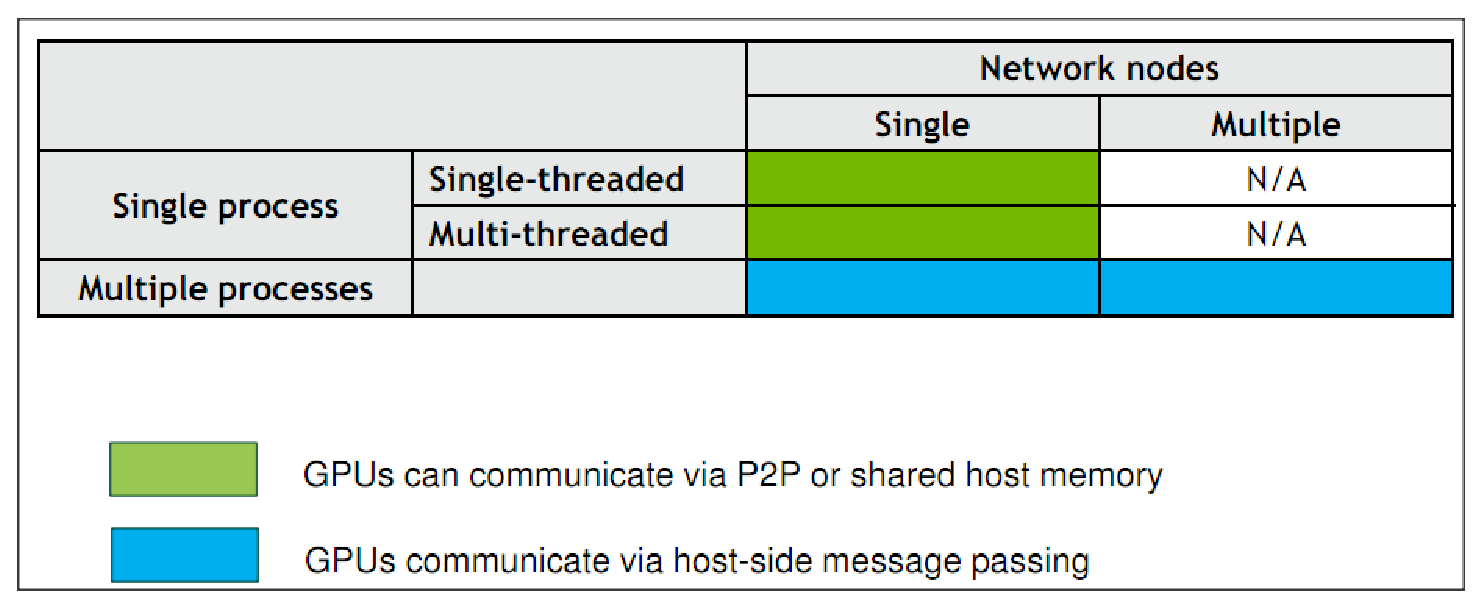
\includegraphics[height=5cm,
    angle=0]{./images/multipleGPU.eps}}
\caption{Summary of how to use multiple GPUs}
\label{fig:case_multipleGPU}
\end{figure}
 
A GPU device is a part of the context and cannot be changed once the context is
established. Thus, a host thread cannot switch form one GPU to another. So you
have the options
\begin{enumerate}
\item Use more than one GPU; yet only one at a time
\item Use multiple GPU at the same time
\end{enumerate}


\section{CUDA + MPI}
\label{sec:CUDA-MPI}

MPI is a standard to exchange data between processes via messages, with APIs 
to exchange messages
\begin{verbatim}
Pt. 2 Pt.: e.g. MPI_Send, MPI_Recv

Collectives, e.g. MPI_Reduce
\end{verbatim}

There are multiple implementations (open source and commercial) of such APIs, under different language binding
\begin{verbatim}
Binding for C/C++, Fortran, Python, ...

E.g. MPICH, OpenMPI, MVAPICH, IBM Platform MPI, Cray MPT, ...
\end{verbatim}

Example: a minimal MPI program
\begin{lstlisting}
#include <mpi.h>
int main(int argc, char *argv[]) {

  int rank,size;

  /* Initialize the MPI library */
  MPI_Init(&argc,&argv);
  
  /* Determine the calling process rank and total number of ranks */
  MPI_Comm_rank(MPI_COMM_WORLD,&rank);
  MPI_Comm_size(MPI_COMM_WORLD,&size);

  /* Call MPI routines like MPI_Send, MPI_Recv, ... */
  ...

  /* Shutdown MPI library */
  MPI_Finalize();
  return 0;
}
\end{lstlisting}

\ref{sec:CUDA-MPI}

\section{Multi-GPU synchronization: cudaStreamWaitEvent}
\label{sec:cudaStreamWaitEvent}

Streams are associated with devices

But cudaStreamWaitEvent can synchronize with events on other GPU: allow
inter-GPU synchronization

\section{Access data from a different GPU}

Sect.\ref{sec:cudaHostAlloc}

\begin{verbatim}
cudaHostAlloc(..., cudaHostAllocPortable)
\end{verbatim}
once such data is allocated, then call cudaHostGetDevicePointer for each GPU


% \section{One at a time}
% \label{sec:one-at-time}
\section{Intel Chipset Architecture}

It's important to know CPU architecture when programming multipe GPUs.
Intel has three main categories of Intel chipsets:
\begin{enumerate}
  \item 4xx series: use PCI bus for interconnection between components. These
  includes: 80486, Pentium, Pentium Pro/II/III, Southbridge 4xx chipsets (using
  PIIX).
  \item 8xx series: use IOH (Hub links) for interconnection between components.
  These includes: Pentium II/III, Pentium III-M (mobile), Pentium 4, Pentium
  4-M/Pentium M/Celeron M, Southbridge 8xx chipsets.
  \item 9xx and 3/4 series: use PCI Express for interconnection between
  components.
  These includes: Pentium 4/Pentium D/Pentium EE, Pentium M/Celeron M, Core/Core
  2 mobile, Core 2, Southbridge 9xx chipsets.
\end{enumerate}
Core 2, and these chipsets use the same design concept,
Fig.\ref{fig:Intel_series4}, in which Front Side Bus (FSB) is used to transfer
the data between CPU and Northbridge which contains a memory controller and
PCI-e graphics controller. In Core 2, Northbridge connect to Southbridge via
Direct Media Interface (DMI).

\begin{figure}[hbt]
  \centerline{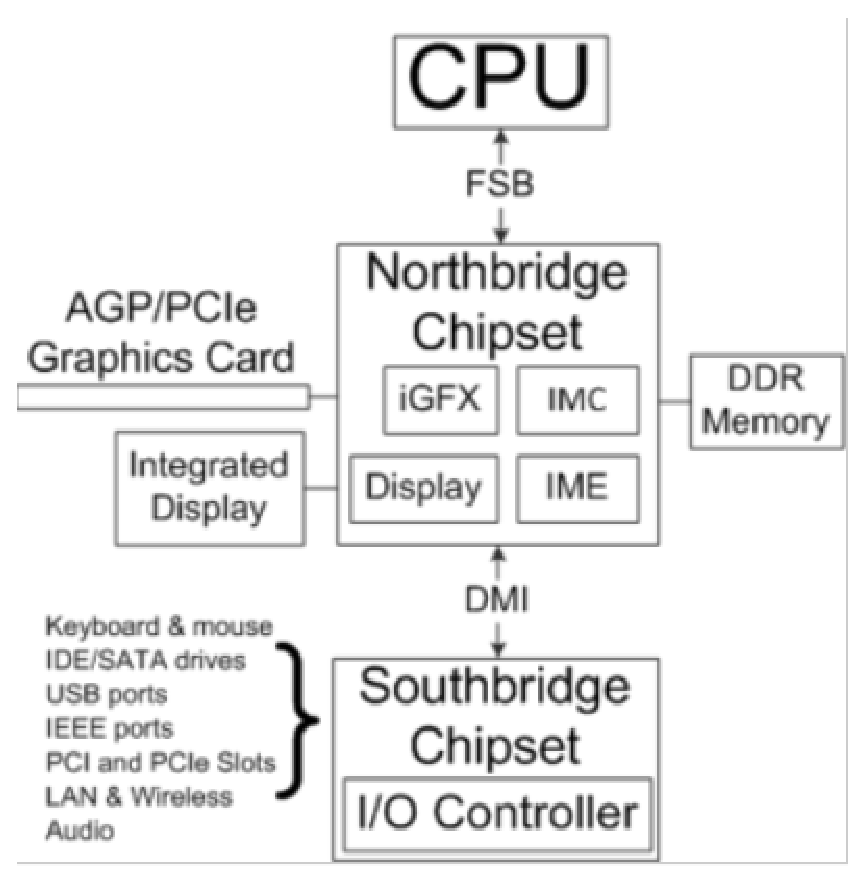
\includegraphics[height=5cm,
    angle=0]{./images/Intel_series4.eps}}
\caption{Front Side Bus (FSB) is heavily used in the design of Intel series 4}
\label{fig:Intel_series4}
\end{figure}

In Southbridge chipsets, CPU connect directly to NorthBridge and use NorthBridge
to interact with high-speed components (RAM, AGP cards). NorthBridge connect to
Southbridge and use it to connect with low-speed components (PCI, USB, ISA, IDE
(harddrive), ACPI, AC'97 (sound controller)). Southbridge is known as {\bf ICH}
(Input/Output Controller Hub), which was later renamed to {\it Legacy I/O
Controller Hub} when Intel introduces Intel X58 I/O hub. PIIX is the predecessor
of ICH, and connect to NorthBridge through an internal PCI bus (133 MB/sec). ICH
uses a proprietery interfact (known as Hub Interface) to connect to Northbridge
with 266 MB/sec.
With ICH in the architecture, Northbridge is called (1) Memory Controller Hub
(MCH), or (2) Graphics and Memory Controller Hub (GMCH) if it has integrated
graphics card connected. There are different version of ICH.
\begin{enumerate}
  \item ICH0 (82801AB):(year 1999) support Ultra ATA/33, 4 PCI slots
  \item ICH (82801AA): support Ultra ATA/66, 6 PCI slots
  \item ICH2 (82801BA) and ICH2-M (82801BAM mobile) : (year 2000) with
  360 pins, support ATA/100, 4 USBs, AC'97 support 6 channel sound
  \item ICH3-S (82801CA server) and ICH3-M (mobile): (year 2001) with 421
  pins, use 6 USB 1.1 (NO version for desktop motherboards)
  \item ICH4 (82801DB) and ICH4-M: (year 2002), support 6 USB 2.0, AC'97
  specification version 2.3
  \item ICH5 (82801EB base), 82801ER (RAID0), 6300ESB (Enterprise Southbridge):
  (year 2003) with 460 pins, support SATA, optionally RAID0, 8 USB 2.0, ACPI 2.0
  \item {\bf ICH6} (82801FB), ICH6-R (RAID), 6311ESB, 6321ESB (Enterprise
  Southbridge with Integrated LAN):  (year 2004) use 4 PCI Express x1 (first
  time), PCI Express x4 (replace Hub Interface giving 1GB/sec), 2 SATA (first
  time), remove PATA, optionally RAID (0,1,0+1, Intel Matrix RAID) 
  
  \item ICH7 (82801GB), ICH7-DH (Digital Home): (year mid-2005) with 2 PCI
  Express x1 slots, SATA (300 MB/sec)
  \item ICH8 (82801HB): (year 2006) with eSATA and Gigabit Ethernet (first time)
  \item ICH9 : (year 2007) remove all PATA support.
  \item {\bf ICH10} (82801JB): (year 2008) 10 Gbits/sec bidireciontal DMI
  (Direct Media Interface) to replace FSB, with 6 PCI Express 1.1, 6 SATA (3Gbits/sec),
  use Intel High  Definition Audio (better than AC'97).
\end{enumerate}



\begin{framed}
Intel Chipset naming convention, e.g. Q55, Q57 
\begin{enumerate}
  \item first character: P=, Q = business-oriented, X=eXtream, H=home user,
  G=with integrated graphics
  \item second character (a numerical): indicate the series
\end{enumerate}
\end{framed}

\begin{figure}[hbt]
  \centerline{
%   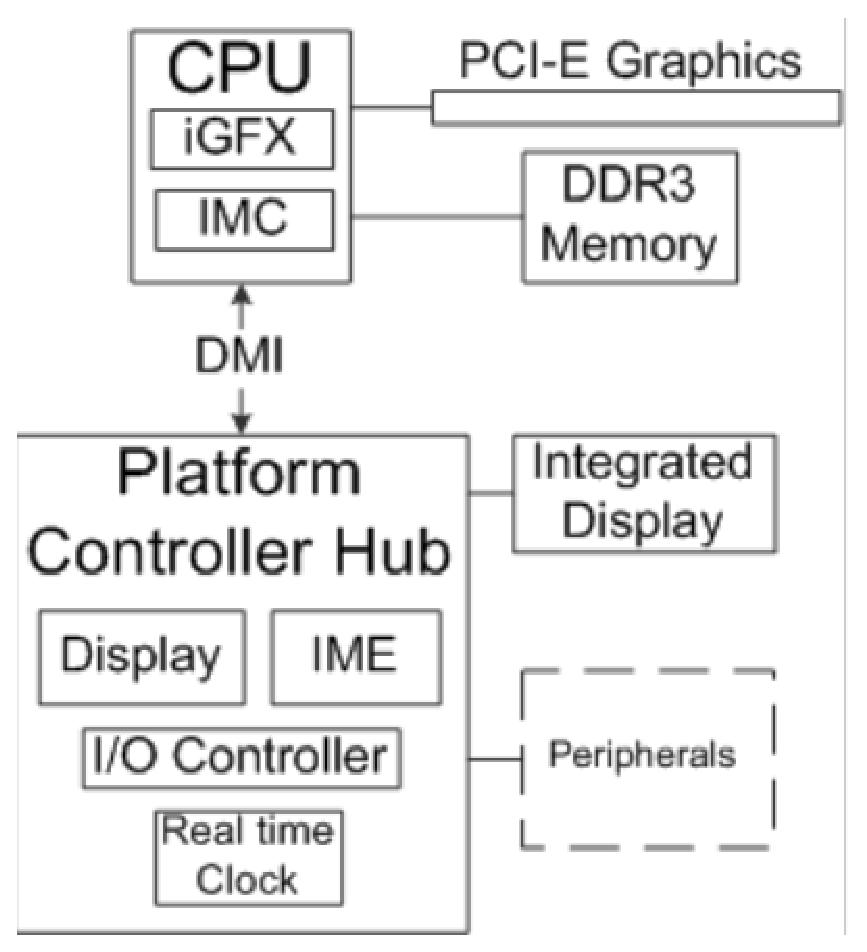
\includegraphics[height=5cm,
%     angle=0]{./images/Intel_i5.eps},
  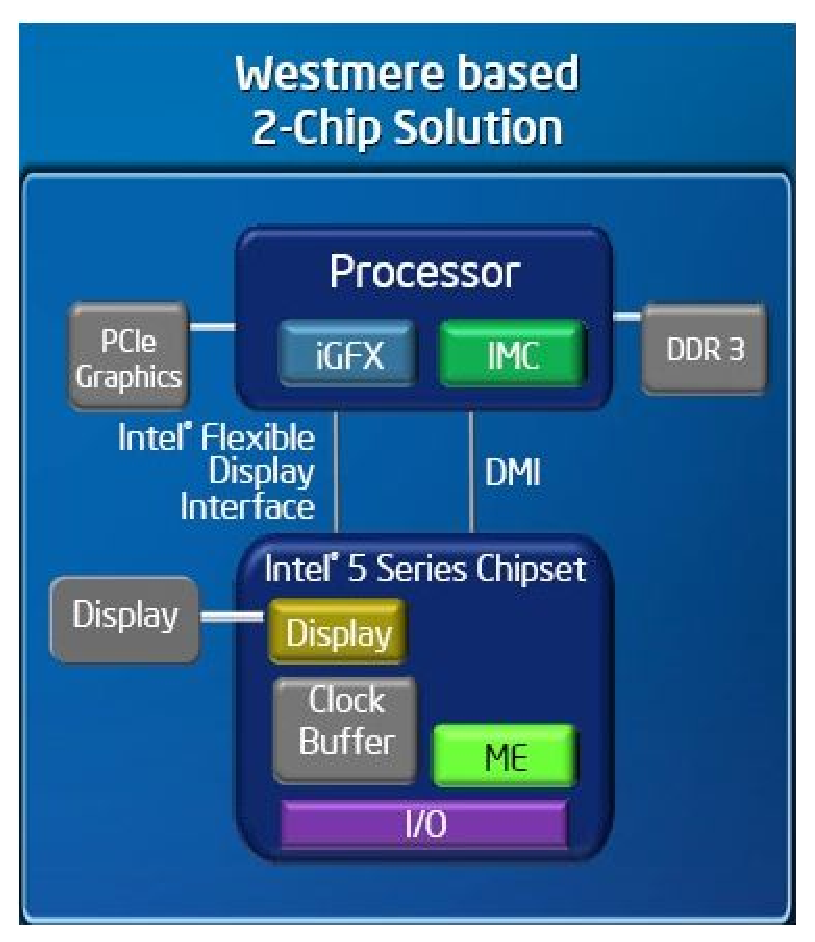
\includegraphics[height=5cm,
    angle=0]{./images/Intel_series5.eps},
    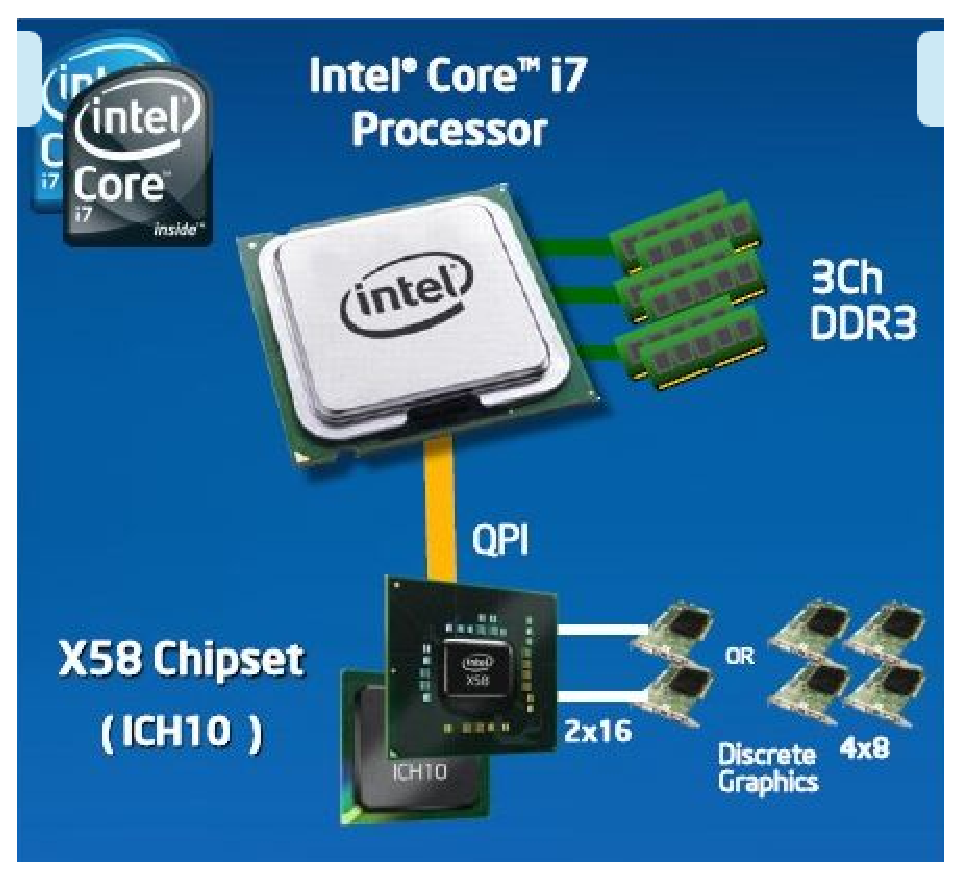
\includegraphics[height=5cm,
    angle=0]{./images/Intel_Core-i7.eps}}
\caption{(A) Intel 5 series design. (B) Intel Core-i7 single socket}
\label{fig:Intel_i5}
\end{figure}

Intel Hub Architecture uses NorthBridge and Southbridge. Since 2008, Intel has
made a significant change in the concept design of motherboard design,
Fig.\ref{fig:Intel_i5}. Memory controller is moved to CPU. FSB is replaced
by Intel QuickPath Interconnect (QPI), e.g. 20-lane QPI link pair with 3.2GHz clock
can deliver the speed of 25.6 GB/sec (double the theoretical bandwidth of 1600
MHz FSB). Intel Core i7 using Nehalem microarchitecture was the first
to use QPI connecting to an X58. QPI can also be used to connect 2 CPUs, first
used in Intel Xeon (March, 2009) and Itanium (Feb 2010). Some lower-end Nehalem
with integrated graphics controller on CPU, it doesn't use QPI, but
DMI instead (2GB/sec or 5GT/s).

\begin{enumerate}
  \item 5/6/7 series: Core i7 introduced in late 2008 with Nehalem
  microarchitecture the basis in Core i7. Core i5 was  introduced in Sept,
  2009; with DMI 2.5 GT/sec; Core i3 introduced in Jan, 2010 for low-end
  proformance processors. Nehalem uses 45nm technology (2008). Westmere is 32nm
  die shrink of Nehalem (2010), with support huge page 1GB in size.
  
  \begin{itemize}
    \item 5 series (Ibex Peak and Tylersburg): Ipex Peak used by Core i5 series,
    with 32nm technology. Northbridge and Southbridge are removed. A new
    component, Platform Controller Hub (PCH) to  provide peripheral 
    connectivity, graphics display with Flexible Display Interface. FSB is
    replaced by DMI. CPU interact directly with PCI Express GPU and DDR3 memory
    for fast access. ICH is integrated into PCH. Intel 5 series uses ICH10/ICH10R.
  Intel 5500 series (Intel 5520, Intel 5500  chipset) use ICH9 or ICH10. 
  
  Intel X58 (Tylersburg) support Core i7, Xeon 5500 series with 45nm technology.
  It doesn't have memory controller hub (MCH), thus is called an X58 I/O hub (IOH, not ICH) and
  function as a Nortbridge to connect with CPU via QPI. X58 uses 40 PCIe lanes.
  X58 QPI can deliver 12.5 GB/sec each direction, and X58 PCI-e 2.0. Dual-socket
  Intel Xeon 5500 series use Tylersburg hub, with QPI connectings 2
  CPUs\footnote{\url{http://www.avadirect.com/intel-nehalem-ep/intel-tylersburg-chipset-motherboards.htm}}.

\begin{figure}[hbt]
  \centerline{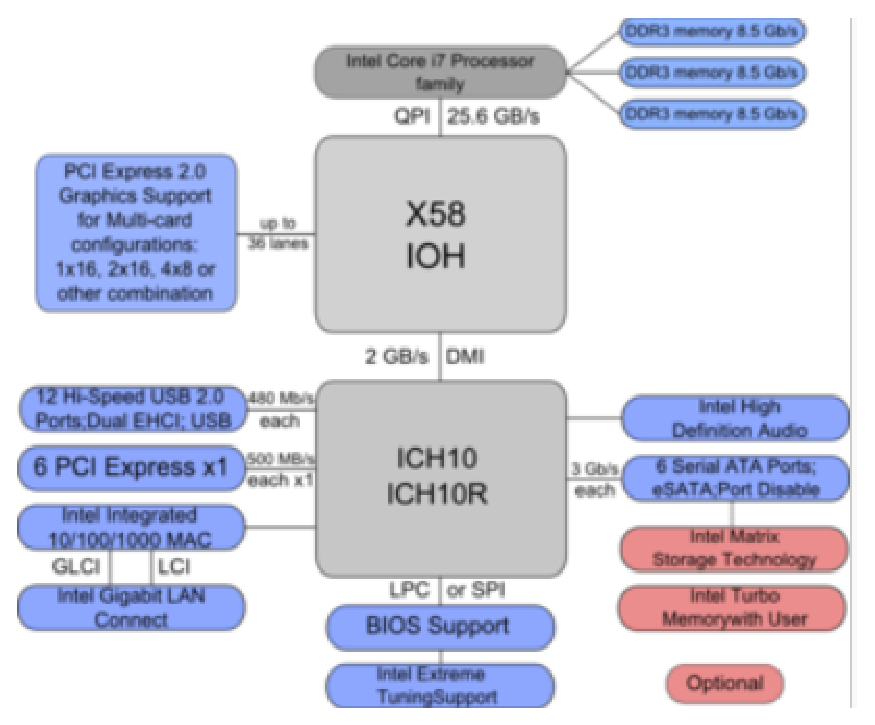
\includegraphics[height=5cm,
    angle=0]{./images/Intel_X58.eps}, \includegraphics[height=5cm,
    angle=0]{./images/Intel_Xeon_5500.eps}}
\caption{Intel Core i7 series design. (B) Intel Xeon 5500 series}
\label{fig:Intel_X58}
\end{figure}
  
    \item Core i 6 series (Sandy Bridge chipsets): use 32nm technology, support
    DDR3-1333 (tested to work with DDR3-2133 also). Built-in GPU has 12
    execution units (EUs).
    
    Sandy Bridge-EN and Sandy Bridge-EP based Xeon E5. 
  
    \item Core i 7 series (Ivy Bridge chipsets: Sandy Bridge CPU is the new
    microarchitecture which is the replacement for previous Pentium families
    (P4,P5, P6, Nehalem). It uses 22nm technology with tri-gate transistors,
    support DDR3-1600, new random number generator RdRand instruction. Built-in
    GPU has 16 EUs, support OpenCL 1.1. Sandy Bridge is 64-bit, quad-core, dual
    threaded, 4 issue, out-of-order microprocessor with new AVX instruction
    (Advanced Vector eXtensions that support 256-bit FP, i.e. 3 and 4 operand).
    
    Ivy Bridge-E processors (2013) to have 12 cores and L3 cache 30MB. Xeon E5
    V2 to replace Xeon E5 Sandy Bridge.
    \end{itemize}
   
  \item 8 series (Lynx Point): use LGA 1150 socket (Socket H3) for Haswell and
  Broadwell microarchitecture, with 6 USB 3.0, 6 SATA 3.0. Intel Xeon C228
  chipset uses LGA 1150 socket. New features: Intel's Transactional
  Synchronization Extensions (TSX) to improve multi-core efficiency.
\end{enumerate}

\begin{framed}
First generation of Intel i7 is based on Nehalem. Next generation of
Intel i7 and Xeon E3 (codename: Ivy Bridge) is based on Sandy Bridge with an
integrated GPU and use 22nm technology (rather than 32nm).
Intel Xeon 5600-series, starting with 6-core (and a few 4-core), is based on
Westmere. Intel Xeon 5500-series, with 4 cores, is based on Nehalem.
AMD has new microprocessor architecture called Interlagos
(Bulldozer)\footnote{dozer architecture uses 2 INT units shared an FP unit in a
single core}, Fig.\ref{fig:SandyBridge_Westmere}, that use Hyper Transport
Technology (25.6GB/s and 16-bit wide link), an alternative to QPI.
\end{framed}

Mordern devices put Northbridge into the CPU die, i.e. System on Chip
processors. Examples are Intel Sandy Bridge architecture and AMD's Fusion
architecture. Intel Haswell (expected available in June 2013) will incorporate
both Northbridge and Southbridge on CPU die for Ultrabook platform. This is
known as {\it Platform Controller Hub}.

    
\subsection{TSX}


\section{QPI and IOH (2 sockets on a mainboard)}
\label{sec:QPI_IOH}

Traditionally, on a machine with 2 CPUs, each connect to a different set of RAM memory.
Programs running on one GPU cannot utilize memory connecting to another CPU.

Modern CPUs also include hardware support for “unified address spaces,” where
multiple CPUs can access one another’s memory efficiently, e.g. Intel's QPI or
AMD's HyperTransport.


QPI is Intel's Quick Path Interconnect technology announced in 2007, and debut
in late 2008. QPI is the interface for point-to-point communication between 2
hardware components. It's the replacement for older technologies, e.g. front-side bus
(FSB), CSI, etc. and is designed primarily for servers and workstations.

\begin{figure}[hbt]
  \centerline{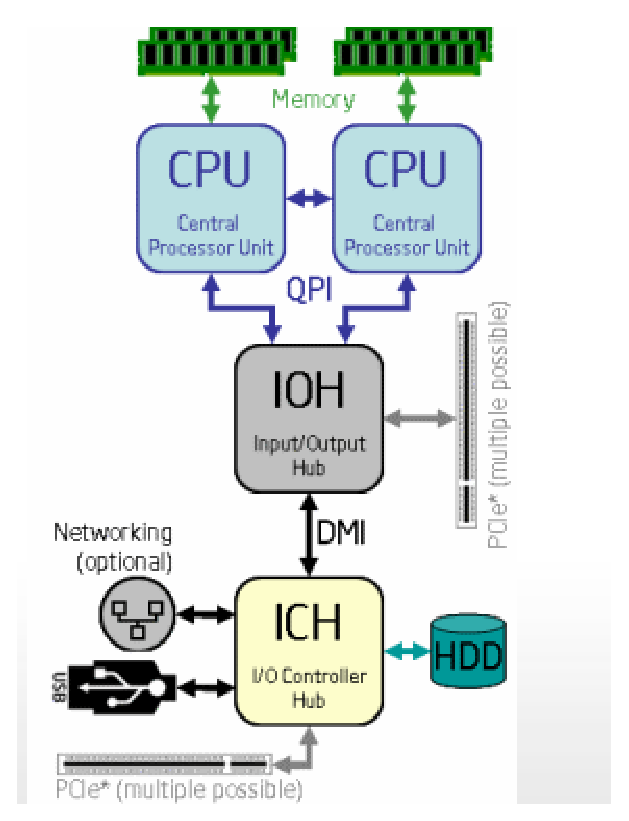
\includegraphics[height=3.5cm,
    angle=0]{./images/QPI_DMI.eps}}
  \caption{Xeon X6550 CPU}
  \label{fig:QPI_DMI}
\end{figure}

\begin{mdframed}
DMI 2.0 links the CPU to peripherals (e.g. memory, graphics card), and with a
much slower rate (5 Gbps (gigabit per second)), Fig.\ref{fig:QPI_DMI}.
\footnote{\url{http://superuser.com/questions/692058/dmi-2-0-vs-8-0-gt-s-qpi}}

QPI is point-to-point, high-speed link between processors only (CPU-CPU,
CPU-GPU). QPI can run at 6.4 GT/s (i.e. 25.6 GB/s using DDR3 1066 MHz) or 8 GT/s
(i.e. 32 GB/s using DDR3 1333 MHz) (Giga Byte per second) depending on which RAM
it connects to. \footnote{\url{https://communities.intel.com/message/125528}}

QPI (Intel) and Hypertransport (AMD) are not buses, but point-to-point
connection. A bus is a set of wires (total 150 wires) that allows several
components to be connected; while a point-to-point is a path connecting ONLY two devices.
\footnote{\url{http://www.hardwaresecrets.com/article/Everything-You-Need-to-Know-About-The-QuickPath-Interconnect-QPI/610}}
QPI provides two separate lanes (total 84 wires), one to read the other one to
write, so they can be done at the same time. This is impossible with buses, as they share the same
lane. Another advantage is that QPI uses less wires than FSB. 

QPI is faster than HyperTransport: maximum transfer rate in Hypertransport is
10.4 GB/s (Phenom processor use HyperTransport at 7.2 GB/s only). This is even
lower due to the limit of CPU transfers of 4 GB/s by AMD Athlon (formerly known
as Athlon 64), Athlon X2 (formerly known as Athlon 64 X2).
\end{mdframed}


QPI can be used to connect 2 processors on a multi-socket motherboard, or a
processor and I/O hub (IOH), or an IOH and another IOH,
Fig.\ref{fig:QPI_connect}. Here, an IOH has 2 QPI channels and 36 PCI-E Gen.2
plus ESI. In Fig.(B), where each CPU connects to its own IOH, the two IOHs need
to connect to each other. Traditionally, the front side bus (FSB) is the memory
bus shared by I/O request and memory access. With the new generation of Intel
CPU, another external memory bus dedicated to memory access only called IMC
(Integrated Memory Controller) which is the bus that connect CPU to the DDR3
memory (Ch0-Ch1-Ch2 given in the figure). The bus that connect CPU to the
external world the QPI. NOTE: \textcolor{red}{As the memory connect directly
to processor via IMC, the IOH now has no memory channels, except a bunch of
PCI-e buses}.

% \begin{framed}
% I/O hub (IOH) is a new term from Intel which refers to Intel X58. 
% 
% \end{framed}

\begin{figure}[hbt]
  \centerline{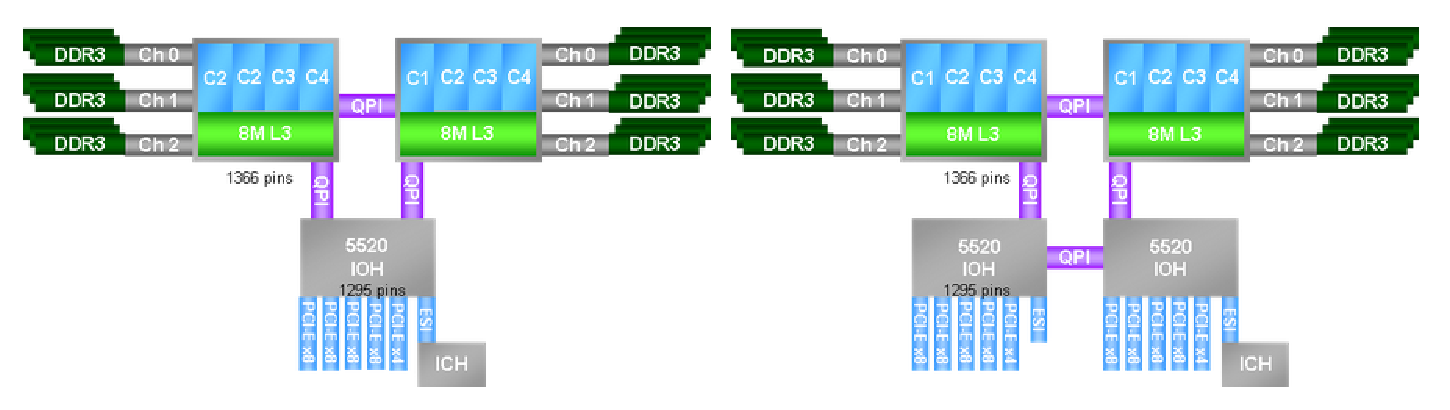
\includegraphics[height=3.5cm,
    angle=0]{./images/QPI_connect.eps}}
  \caption{(A) A 2-socket system with a single IOH, (B) A 2-socket system
  with 2 IOHs. NOTE: C1-C4 = core index, Ch0-Ch2 = integrated memory
  controller, support DDR3}
  \label{fig:QPI_connect}
\end{figure}

Each lane in QPI can transfer 20 bits per time. In these 20 bits, 16-bits are
used for transfer data, and the remaining 4 bits are for correction code (CRC -
Cyclical Redundancy Check). In addition, QPI can treats each 20-bit lane as four
5-bit lanes, Fig.\ref{fig:QPI_5bit-lanes}. This division is to improve
reliability, especially on server market environment (which is thus not
available on desktops). This allows the system to shut down the portion of the
lane that is physically damaged. The transfer rate is reduced, but the system
won't fail.

\begin{figure}[hbt]
  \centerline{\includegraphics[height=3.5cm,
    angle=0]{./images/QPI_5bit-lanes.eps}}
  \caption{QPI can run at four 5-bit lanes }
  \label{fig:QPI_5bit-lanes}
\end{figure}

The first version, QPI 1.0, works at the clock rate
3.2 GHz, and transfering two data per clock cycle (DDR - double data rate),
making the bus to work as if it's 6.4 GHz clock rate. However, Intel uses a
different concept, called GT/s (GigaTransfer per second). GigaTransfer refers to
the amount of data transfered (not only data, but also the bits that are lost
as a result of interface overhead). 
\begin{verbatim}
6.4 GHz x 16 bits / 8 = 12.8 GB/s (each QPI lane)

 = 25.6 GB/s (two data-path QPI read+write)
\end{verbatim}

QPI provides 3 different power modes: L0, L0s and L1. 
\begin{itemize}
  \item L0: QPI fully functional
  \item L0s: the data wires and the circuits that drives these wires are turned
  off
  \item L1: everything is turned off, in return for a higher wake-up time.
\end{itemize}


On a desktop system, typically, there's a single socket on the mainboard. Core
i7 (Nehalem architecture processor) has a single QPI channel, yet Xeon 5500
(April, 2009) has 2 QPI, i.e. 2-sockets mainboard. Each socket fit to a single
processor. Processors based on QPI are Nehalem, Westmere, and Tukwila families.

\begin{verbatim}
The rate is calculated as
    3.2 GHz
    x 2 bits/Hz (double data rate)
    x 20 (QPI link width)
    x (64/80) (data bits/flit bits)
    x 2 (unidirectional send and receive operating simultaneously)
    / 8 (bits/byte)
    = 25.6 GB/s 
\end{verbatim} 
QPI bandwidth is 12.8GB/s per direction, giving 25.6GB/s bi-direction. ``Each
PCI-E Gen 2 lane operates at 5Gbit/sec for a net bandwidth of 500MB/s per lane,
per direction. A x4 PCI-E Gen 2 channel is rated 2GB/s per direction, and 4GB/s
per direction for the x8 channel. So while the 36 PCI-E Gen2 lanes on the 5520
IOH are nominally rated for 18GB/s per direction, the maximum bandwidth per QPI
is still 12.8GB/s per direction''.

\begin{figure}[hbt]
  \centerline{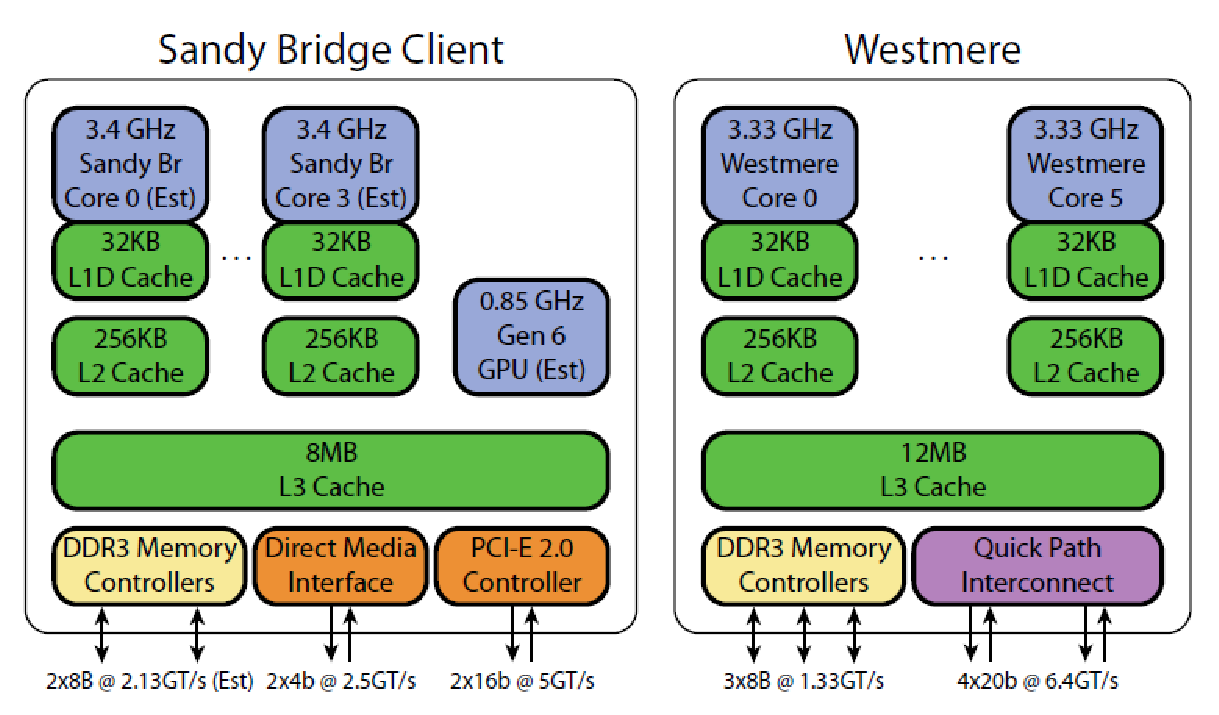
\includegraphics[height=5cm,
    angle=0]{./images/sandybridge_westmere.eps}}
  \caption{Sandy Bridge and Westmere}
  \label{fig:SandyBridge_Westmere}
\end{figure}

First generation of QPI 1.0 runs at 6.4 GT/s, with 20 lanes of high-speed PCI-E
2.0 and 20GB/s of bandwidth, in which 4 lanes are dedicated to DMI (Intel's Direct Media
Interface). GPUs and RAID controllers can be connected directly to the CPU. It
also has enough PCI-E lanes to handle dual-GPU configuration (or a GPU and a
high performance network card or storage controller). In this version, it has
QPI in the consumer part, Fig.\ref{fig:QPI_1.0}. Nehalem-EP/EX, Westmere-EP/EX
and Tukwila use QPI 1.0.

The second generation QPI 1.1 is an increment enhancement at physical (run at
higher frequencies) and logical layer (use only home snooping protocol, remove
source snooping), to run at 6.4 GT/sec, 7.2GT/sec, or 8GT/sec. QPI 1.1 is mainly
designed for 2-socket servers, and is backward compatible with QPI 1.0. Sandy
Bridge-EP and the Romley platform (two-socket Sandy-Bridge-EP based server line)
will be the first products to use QPI 1.1, followed by Ivy Bridge-EP/EX.

\begin{figure}[hbt]
  \centerline{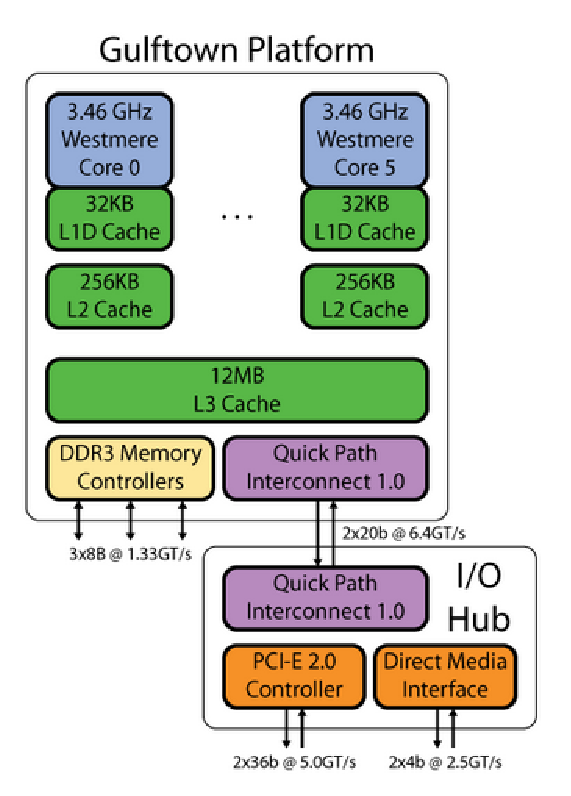
\includegraphics[height=5cm,
    angle=0]{./images/QPI_1.0.eps}}
  \caption{QPI 1.0}
  \label{fig:QPI_1.0}
\end{figure}


\begin{enumerate}
  \item \url{http://www.realworldtech.com/qpi-evolved/}
  \item \url{http://www.realworldtech.com/common-system-interface/2/}
  \item
  \url{http://www.qdpma.com/systemarchitecture/systemarchitecture_qpi.html}
\end{enumerate}





\section{SLI}
\label{sec:SLI}

Nvidia Scalable Link Interface (SLI) is a technology that links multiple GPUs on
the same machine to improve graphics performance, i.e. rendering, by dividing
the workload across multiple GPUs.

Two GPUs must be attached to two PCI-e x16 slots, and linked together using
external SLI bridge connectors. SLI is enabled via Nvidia control panel. Then,
the driver can treat both GPUs as a single logical device, and divide the
workload automatically depending on the selected mode. There are 5 modes: 
\begin{enumerate}
  \item AFR = alternate frame rendering, i.e. frame even is done by GPU0, frame
  odd is done by GPU1 (preferref mode, whole frame is done by a single GPU at a
  time, and thus requires little inter-GPU communication)
  \item SFR = split frame rendering, i.e. a frame is splitted into, say
  2, regions, each region is processed by a single GPU. Boundary processing is
  required, i.e. some of the works is duplicated, and communication overhead is
  higher. 
  \item Boost Performance Hybrid SLI: this mode is somehow similar to AFR mode,
  however, one will do more frames before switching to another. This scenario
  work wells when you have one powerful GPU, and the other is at a lower entry. 
  \item SLIAA : improve antialiasing, but not performance level. The setting is
  in ``Antialiased settings'', which can be SLI8x or SLI16x (if two GPUs are
  used), and SLI32x (if 4 GPUs are used).
  
  \item Compatibility mode: default setting for all aplications that don't have
  SLI profile. Here one GPU is being used for display, the other ones can be
  either idle, or in use by other applications or on a separate device. 
\end{enumerate}

The choice of an appropriate mode is based on SLI profile, which can be created
for a single application by sending it to nVidia. Then, in the next release of
the driver, the profile of your application will be included, making it
available to end-users. If your application doesn't have an SLI profile, a good
choice is to use SLIAA mode.

\textcolor{red}{An important using SLI is that data are duplicated in all GPUs
involved. So, using two GPUs, each with 512MB, we also have total 512MB for
video displays}. Similarly, when using CUDA on SLI technology, an allocation in
one CUDA device on one GPU will consume more memory than on other GPUs that are
part of SLI configuration. 

Also, each GPU on the SLI configuration requires a separate CUDA context. To
identify the CUDA device handle for the device being used for rendering in the
current and next frame. 




\section{GPUDirect}
\label{sec:GPUDirect}

\begin{enumerate}
  \item GPUDirect v1 (introduced for CUDA 4.0 with IB
  HCAs - Sect.\ref{sec:GPUDirect-v1} )
  
  
  \item GPUDirect v2 = GPUDirect peer-to-peer (introduced for CUDA 4.0 with IB
  HCAs on UVA feature of Fermi-class GPU - Sect.\ref{sec:GPUDirect-v2} )
  
  for transfer of data between two CUDA GPUs on the same PCIE fabric only. It
  does not enable interoperability with any other kind of device.
  
  
  \item GPUDirect v3 = GPUDirect RDMA (introduced for Kepler-class GPU -
  Sect.\ref{sec:GPUDirect-v3}:
  between a GPU with any third-party device, with constraint: two device must be on the same PCIExpress root
  
  
  \item 
\end{enumerate}


\section{Multi-GPU CUDA 3.2 and earlier }
\label{sec:multi-GPU_3.2}

\subsection{CUDA runtime API 3.2 or earlier {\it per se}}
\label{sec:one-a-time_CUDA3.2-runtime}

Impossible.



\subsection{CUDA driver API 3.2 or earlier}
\label{sec:one-a-time_CUDA3.2-driver}

Even though we can only use one GPU at a time, we can return to using the device
after switching to another one via push/pop context function
\verb!cuCtxPushCurrent/ctxCtxPopCurrent! (Sect.\ref{sec:GPUs_driverAPI4.0}). By
doing this, indeed, a single GPU can be
  used at a time, though during the runtime, the host thread can switch from one
  GPU to another.
  

\subsection{CUDA 3.2 runtime with MPI}
\label{sec:GPUs_cuda32.MPI}

One CUDA context is created per CPU thread; and one CPU thread can use
only one CUDA context. Different CPU thread cannot share CUDA context;
which is a huge limitation.

So, to use multiple GPUs, we need one CPU thread per device. At a
result, one thread cannot do any thing with GPU data from other CPU
thread. So, the only way is to create a ``proxy pattern'' that allow
one thread to tell another thread to get the data back to host memory
for the thread to use. 

To prevent data races, we need to use barriers/metaphores in MPI. So,
the common model is to have a main host thread to do I/O data to
permanent data storage (harddrive), and control other slave host
threads. The slave host threads do (1) copy data to/back device, (2)
launch kernel. The data is split into as many chunk as many GPU devices

\begin{verbatim}
tokens{
   thread_t threadID
   int id;
}
\end{verbatim}
contains the thread ID and the GPU id that the thread use. Example:
\verb!vecadd()! is the slave host thread.

So, the main limitation is that each host thread can only access to
the memory objects that it allocates. 

Semaphore: when a data already copy to the device, the thread that
create that memory address, can enable the semaphore, telling other
thread can get access to the data; but still need this thread to do
the copy back. Page-locked memory buffers may be used to store the
data copied back, and can be very big.

QUESTION: How we know the limitation of page-locked memory in a
machine? (TUAN)


% \subsection{MPI}
% \label{sec:mpi}


\verb!data_server()! is the node to do the data allocation, 

In the data stencil example, each node use a subvolume of the
data. Suppose, the whole z-dimension is not splitted; only along the
xy-plane. There is overlapped between the subvolume, i.e. 2 slices on
the left and 2 on the right, so totally 4 increment of data it really
process.

\begin{figure}[hbt]
  \centerline{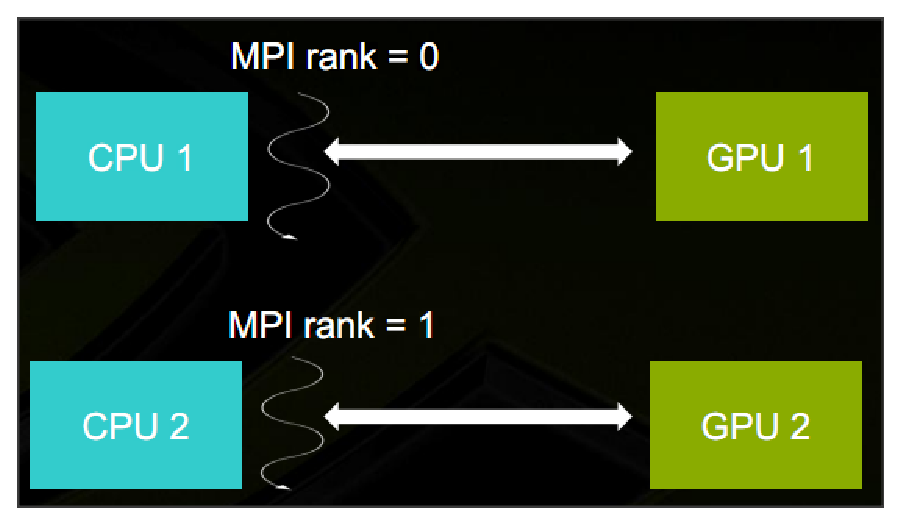
\includegraphics[height=5cm,
    angle=0]{./images/MPI_GPU.eps}}
\caption{MPI and CUDA}
\label{fig:MPI_GPU}
\end{figure}


To increase the performance, Compute the boundary that the next thread
need to use first; and during the time it switch, the kernel will
compute the other part of the subvolume.

By default, data allocated on host is for synchronous data
transfer. So, we need to use \verb!cudaMallocHost()! to allocate host
memory for ghost data and can be used for asynchronous data transfer.


Here, using Infiniband, the data from GPU is internal copy (not seen
by user) between CUDA buffers and Infiniband buffers.

\subsection{XMP}
\label{sec:GPUs_XMP}

\begin{verbatim}
#pragma xmp nodes p(*) // node declaration
#pragma xmp nodes gpu g(*) // GPU node declaration
...
#pragma xmp distribute AP() onto p(*) // data distribution
#pragma xmp distribute AG() onto g(*)
#pragma xmp align G[i] with AG[i] // data alignment
#pragma amp align P[i] with AP[i]
int main(void) {
...
#pragma xmp gmove // data movement by gmove (CPU=>GPU)
AG[:] = AP[:];
#pragma xmp loop on AG(i)
for(i=0; ...) // computation on GPU (passed to CUDA compiler)
AG[i] = ...
#pragma xmp gmove // data movement by gmove (GPU=>CPU)
AP[:] = AG[:];
\end{verbatim}

References:
\begin{itemize}
\item P2S2-2010 Panel Is Hybrid Programming a Bad Idea Whose Time Has
  Come? - Taisuke Boku. 2010
\end{itemize}

\subsection{CUDA 3.2 runtime with pthreads}
\label{sec:GPUs_pthreads}


The trick using multiple GPUs with CUDA runtime APIs is that each GPU needs to
be controlled by a single CPU thread. First we create a structure
\verb!DataStruct! that contains the information about the device we want to use
as well as the data it will process, and pass it to an entry function that
create a new CPU thread \verb!start_thread()!. Typically, we have 2 GPUs on a single machine, so we create an array of 2
elements.
\begin{lstlisting}
DataStruct data[2];

data[0].deviceID = 0;
data[0].size = N/2;
data[0].a = a; //point to the starting data address
data[0].b = b;

data[1].deviceID = 0;
data[1].size = N/2;
data[1].a = a+N/2; // point to the starting data address
data[1].b = b+N/2;
\end{lstlisting}
The function \verb!start_thread(func_name, &(data[i]))! create a new thread
which then calls to the specified function \verb!func_name! and pass the
DataStruct information to it.
\begin{lstlisting}
CUTThread  thread = start_thread ( func_name, &( data[0]));
func_name ( & (data[1])); // we don't have to create a new thread for this
\end{lstlisting}
In the main program, if it need to get the data from the newly created thread,
we call
\begin{lstlisting}
end_thread(thread);

/// free data
free(a);
free(b);
\end{lstlisting}

This is how we define the routine \verb!func_name! to do what we need
\begin{lstlisting}
void* func_name ( void *pvoidData) {
  DataStruct *data = (DataStruct*) pvoidData;
   // each thread call a device, using a different ID
  HANDLE_ERROR( cudaSetDevice ( data->deviceID));
  
  // the body of the function is the same as the original one,
  // except the starting point of data need to be different
  
  a = data->a;
  b = data->b;
  ..... // the next step should be the same
  
\end{lstlisting}

There are many applications where you need to share the data between GPUs, e.g.
stencil computation when each GPU does the calculation for a subset of data,
there should be a mechanism to exchange data. Also, if your simulation iterate
hundreds of thousands of loops, you don't want to create and destroy a CPU
thread each time, but keeping it during the whole simulation. This requires more
interference from programmer side. 

\subsection{OpenMPI}
\label{sec:GPUs_openMPI}


\begin{figure}[hbt]
  \centerline{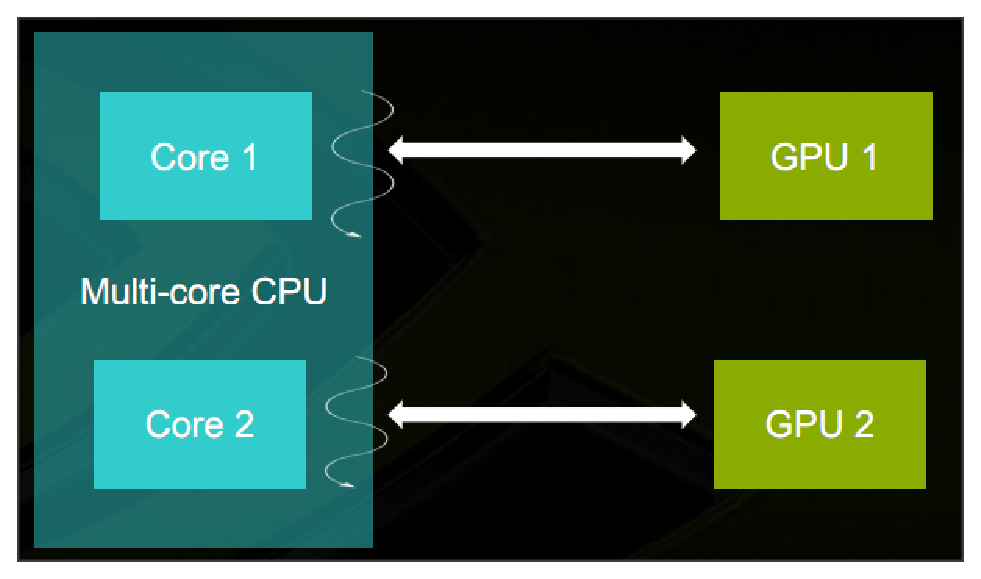
\includegraphics[height=5cm,
    angle=0]{./images/OpenMP_GPU.eps}}
\caption{OpenMP and CUDA}
\label{fig:OpenMP_GPU}
\end{figure}

GPU communications used 'pinned' buffers for data movement. Optimizations such
as write-combining with overlapping GPU computation and data transfer can be
done to achieve faster performance. 


\subsection{GMAC}
\label{sec:GPUs_gmac}

GMAC = Global Memory Access 

\url{http://code.google.com/p/adsm/wiki/API}

Based on a unifired CPU/GPU virtual address space. A memory data can
be accessed by both the CPU or GPU using the same pointer. 


\verb!gmacPtr()! only need for CUDA 3.x; not in CUDA 4.x. The reason
is that in CUDA 4.0, a CPU host thread can get access to GPU data
allocated by any other CPU host threads. However, it's important to
know that, a GPU kernel can only get access to the data allocated by
the host thread which it's bound to.

\subsection{GPUDirect 1.0 + Infiniband + MPI}
\label{sec:GPUs_GPUDirect1}

\textcolor{red}{Since Infiniband HCA ConnectX-2 (Sect.\ref{sec:Mellanox_cards}),
GPUDirect is supported.}


\textcolor{red}{GPUDirect 1.0} was first released with CUDA 3.1 (June 2010) and
is better with CUDA 4.0. It is designed for application that communciate over a
network or on the same machine using Mellanox ConnectX card with MPI programming
model. It's a joint effort between Nvidia and Mellanox. This allows
third-parties network/storage devices to direct access CUDA memory. This
eliminates unncessary sys mem copy \& CPU overhead, as data no need to go
through CPU DRAM before passing to Infiniband network. This improves upto 30\%
in communication performance.

In CUDA 3.1 and 3.2, GPU and Infiniband communicate by using a shared 'pinned'
buffers (or page-locked buffer) for efficient RDMA transactions. One kernel copy
the data to the 'pinned' buffers, and the other kernel using a different GPU can
access this data thanks to zero-copy data transfer, i.e. the kernel can access
CPU 'pinned' data without copying to GPU global memory.

\begin{figure}[hbt]
      \centerline{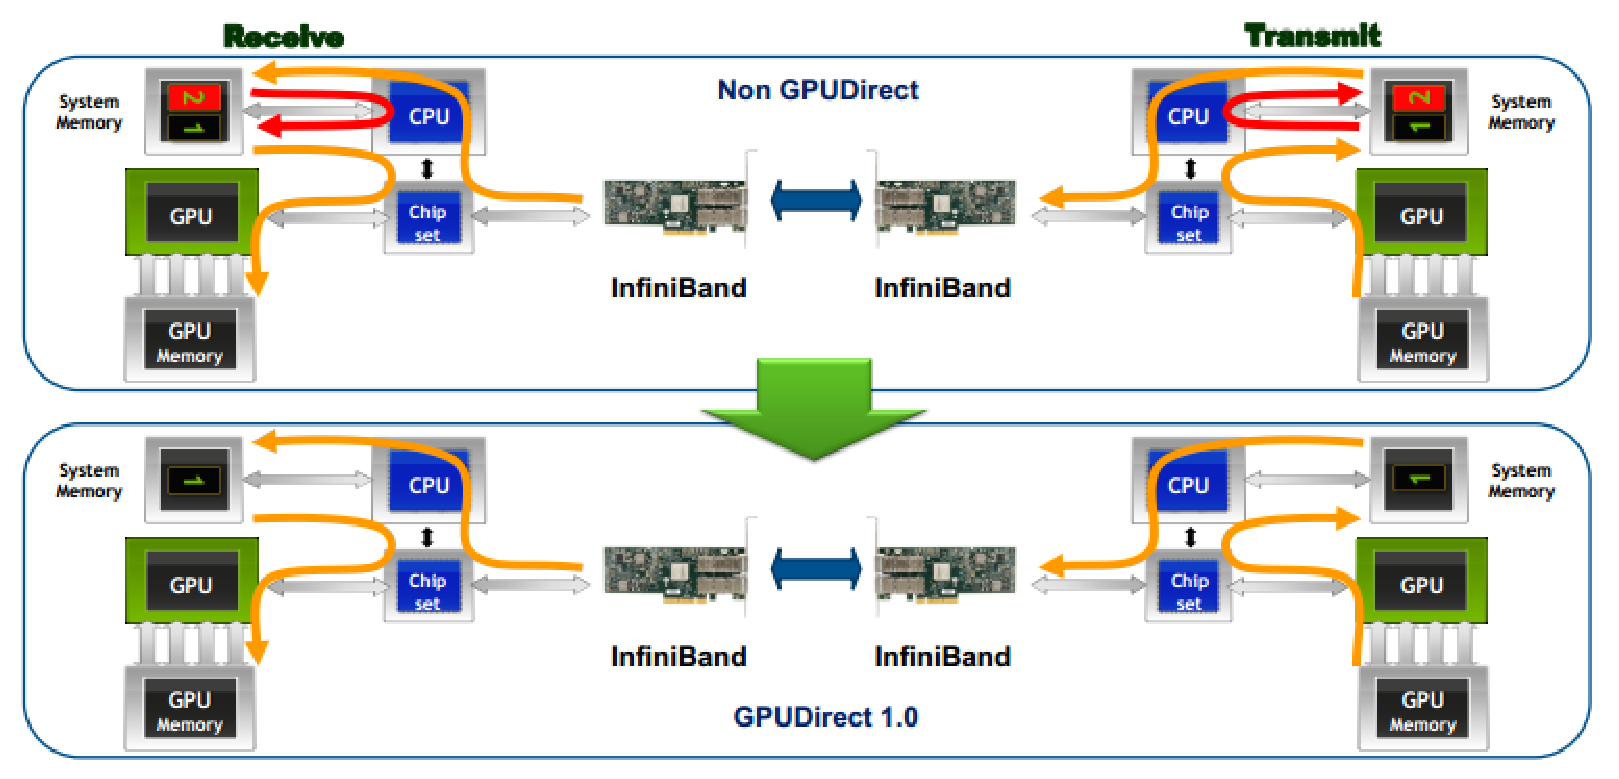
\includegraphics[height=5cm,
    angle=0]{./images/GPUDirect_1.0.eps}}
\caption{Without GPUDirect 1.0, two copies is required for inter-node
communications. With GPUDirect 1.0, only one copy from GPU to 'pinned' memory,
and then Infiniband can access from that}
\label{fig:GPUDirect1}
\end{figure}


Infiniband vendors first support GPUDirect are Mellanox and QLogic.
\textcolor{red}{The first requirement to use GPUDirect is that we need to use
pinned-memory.} Without GPUDirect support, first the data is copied from GPU
memory to CPU pinned-memory sysmem1 which cannot be accessed from Infiniband
devices. Instead, CPU need to copy sysmem1 to a new location sysmem2, where
Infiniband can get access to. With GPUDirect support, Infiniband can get access
to sysmem1 directly usinng remote direct memory access RDMA; so we can avoid one
unnecessary memory copy.

% Without GPUDirect, what the Infiniband driver doing is to allocate
% some buffers, actually 2: one is being used by the Infiniband...

With GPU Direct enabled, Infiniband can do the copy data directly from 'pinned'
buffer to the Infiniband. So, it removes a number of intermediate data copy
steps. However, notice that there is noway for the Infiniband to retrieve the
data directly from GPU, so you cannot pass a pointer to the MPI function.
Instead, you need to copy it back to the host memory fist.

Peer-to-peer GPU data copy without passing to the host memory require
both GPUs to use the same PCI address bus on the same
machine. Otherwise, this cannot happen. 

\begin{enumerate}
  \item Fermi-based GPUs
  \item IB software: OFED 1.5.x with GPUDirect support (Sect.\ref{sec:OFED})
  \item MPI: MVAPICH 1.5+
  \item NVIDIA driver 256.35 and above
  \item NVIDIA driver 3.2+ (including OpenCL driver)
\end{enumerate}


\section{Multiple CUDA 4.0 }
\label{sec:multi-GPU_CUDA4.0}

CUDA 4.0 make it easire to work with multi-GPUs on (1) a single node, (2)
across the network
\begin{enumerate}
\item within node: use runtime (Sect.\ref{sec:GPUs_cuda4_singlethread}) and
driver API (Sect.\ref{sec:GPUs_driverAPI4.0})
\item GPUDirect 2.0
(Sect.\ref{sec:GPUs_GPUDirect2})
\end{enumerate}

\begin{figure}[hbt]
  \centerline{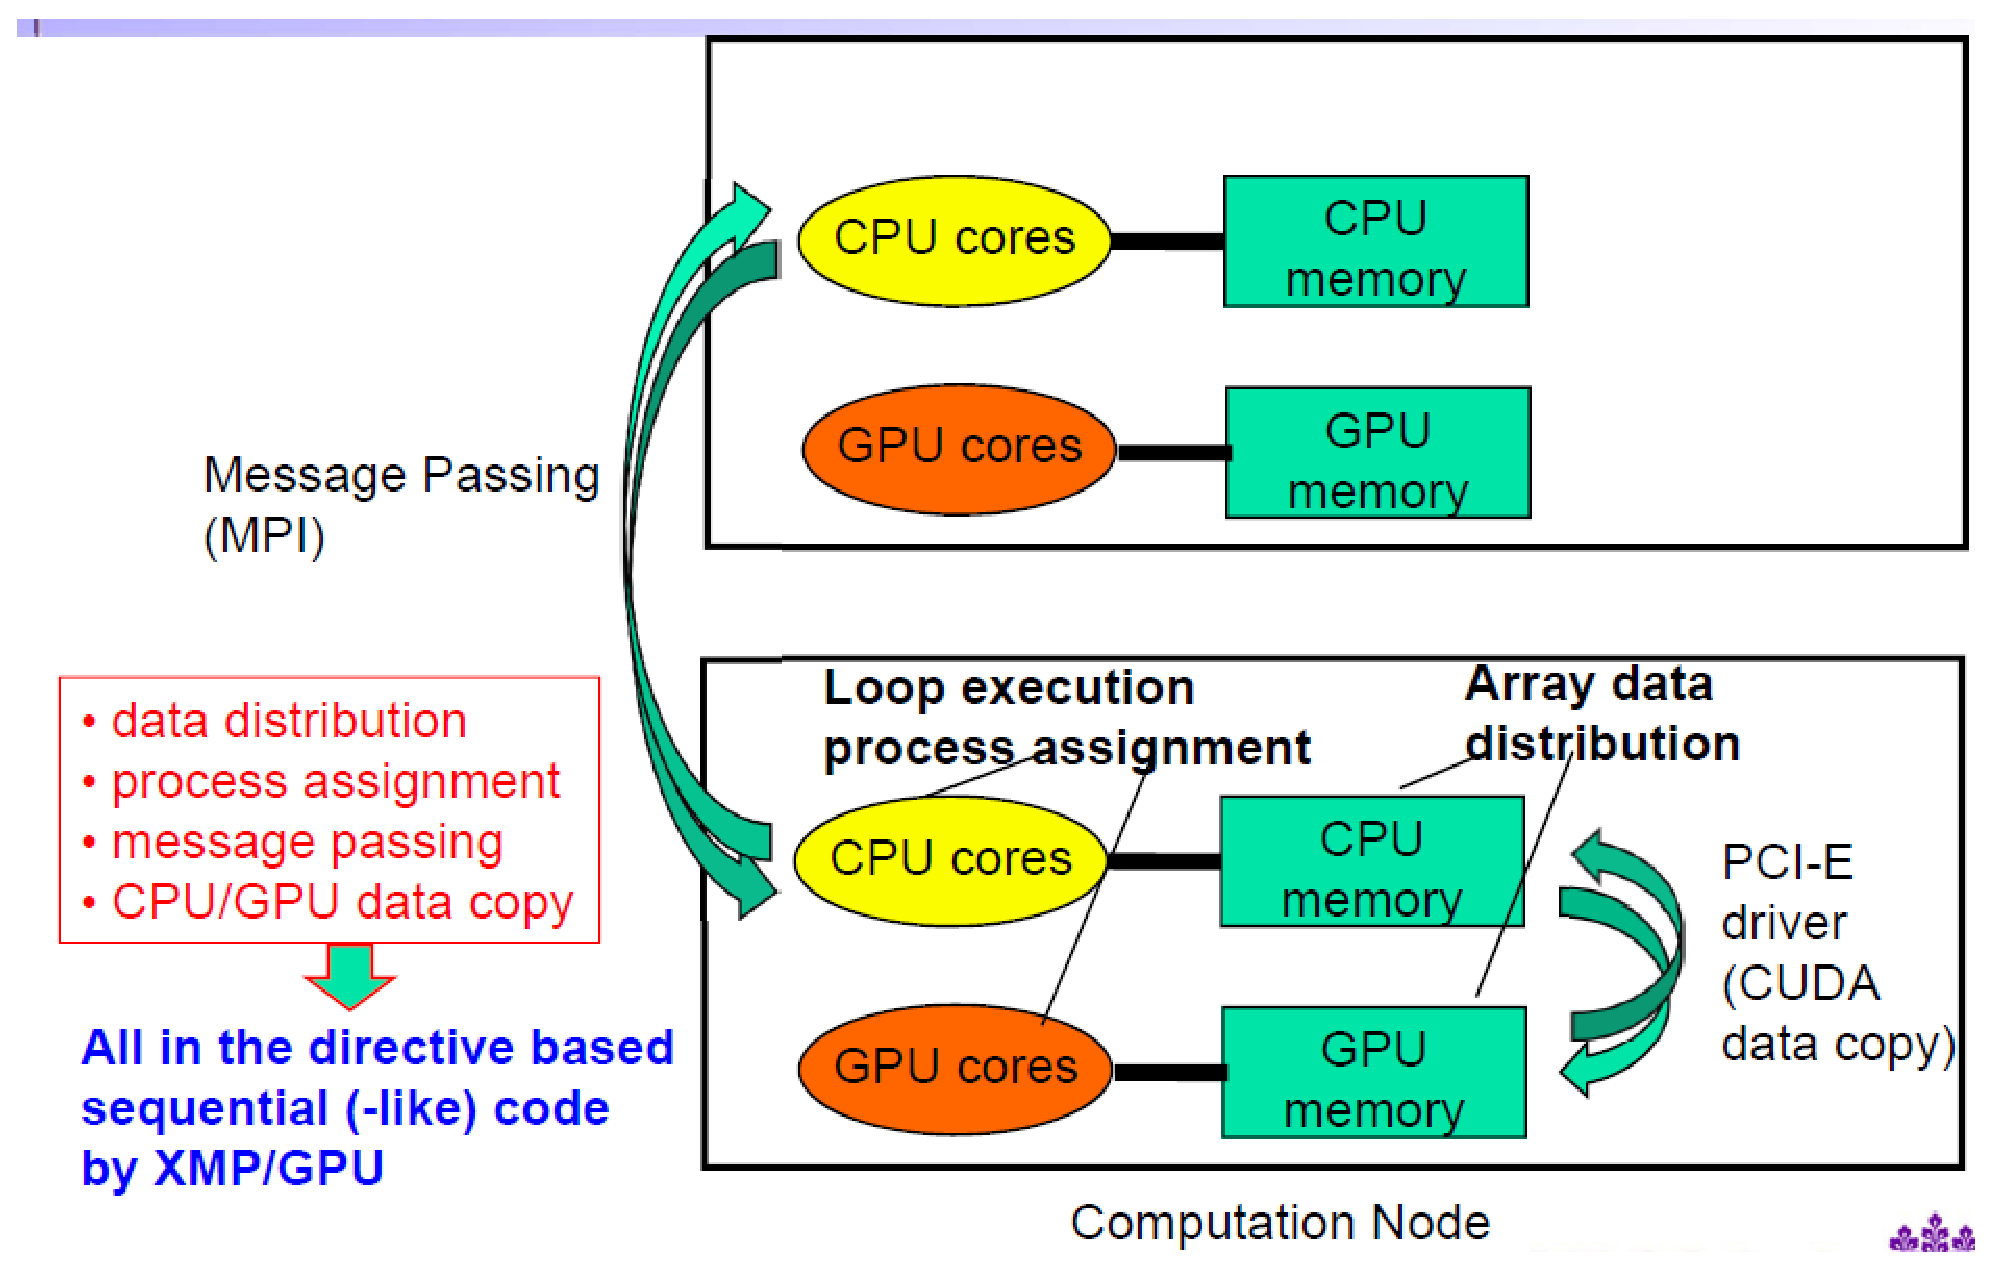
\includegraphics[height=5cm,
    angle=0]{./images/multiple_GPU_CPU.eps}}
  \caption{CPU/GPU coordination data management}
  \label{fig:GPU_CPU}
\end{figure}

\subsection{CUDA runtime 4.x (single host thread)}
\label{sec:GPUs_cuda4_singlethread}

In CUDA 3.2 and earlier, you can call cudaSetDevice() only once. CUDA 4.0 now
relaxed this restrion, allowing to switch from one device to another by calling
it multiple times thanks to UVA (Sect.\ref{sec:UVA}). In CUDA model, there is
only one CUDA context per device and one CUDA stream per CPU thread and device.
Once a CUDA context is created, we cannot change the GPU. However, with UVA, the
single CUDA context can be used for both GPU1 and GPU 2.

Using UVA in Fermi-based GPU, CUDA 4.x allow one CPU host thread to switch the
CUDA stream and CUDA context. NOTE: it works for multiple GPUs on a single
machine. GPU have consecutive IDs, starting with 0. We can use device management
calls
\begin{enumerate}
\item cudaGetDeviceCount( int *num\_devices )
\item cudaSetDevice( int dev1 )
\item process data on device first
\item cudaSetDevice(int dev2)
\item process data on device second
\item cudaGetDevice( int *current\_device\_id )
\item go back withstep 2
\end{enumerate}
As one thread can now work with multiple GPUs, CUDA runtime API
starting with \verb!cudaThread...!, e.g. \verb!cudaThreadExit()!, need to be
changed to a new name that match its function. So, from CUDA 4.0, the new
prefix is \verb!cudaDevice...!, e.g. \verb!cudaDeviceReset()!,
\verb!cudaDeviceSynchronize()!. 

When you querying the properties of a device, no context is created. 
\begin{lstlisting}
cudaGetDeviceProperties(cudaDeviceProp *properties, int
          device_id)
\end{lstlisting}

% Before a context creation, you can select the device
% \begin{lstlisting}
%  cudaSetDevice(...)
% \end{lstlisting}
% with the chosen device ID. In Fortran CUDA, the system will
% automatically detect the available device and the context is
% automatically created when the program run, so programmer cannot
% choose the device. One can force a context creation by calling
% \begin{lstlisting}
% cudaFree(0)
% \end{lstlisting}



\begin{lstlisting}
// Run independent kernel on each CUDA device
int numDevs = 0;
cudaGetNumDevices(&numDevs);
...
for (int d = 0; d < numDevs; d++) {
  cudaSetDevice(d);
  kernel<<<blocks, threads>>>(args);
}
\end{lstlisting}

CUDA 4.x makes it easier to use multiple GPU from a single CPU thread
by calling \verb!cudaSetDevice(int n)! to switch to a device it want
to use; and then you can call copy data from the device. As on a
single host thread, we need to use critical sections to prevent data
races.

\begin{lstlisting}
cudaSetDevice(0);      // start on device 0
cudaMalloc(&p0, size); // allocate memory for p0 on device 0
K0<<<1,1>>>(p0);       // launch kernel K0 on device 0


cudaSetDevice(1);      // switch to device 1 (Not legal in CUDA 3.x!)
cudaMalloc(&p1, size); // allocate memory for p1 on device 1
K1<<<1,1>>>(p1);       // launch kernel K1 on device 1
\end{lstlisting}

\begin{framed}
IMPORTANT: All CUDA calls are issued to the {\bf current} (selected) GPU, with
the exception of asynchronous peer-to-peer communication that allows you to
copy data betweeen 2 GPUs or get access to data from another GPU not necessarily
a ``current'' one.

Asynchronous calls (kernel, memcopies) don't block the switching of GPU. This
allows code on different GPUs to run concurrently.
\end{framed}

You can also combine with using CUDA streams and events to synchronize between
GPUs (Sect.\ref{sec:GPUs_device-coupling}). However, it's important to know that
you cannot evoke a kernel, using the stream not from the active GPU. The folling
code is wrong, Fig.\ref{fig:CUDA4_wrongstream}.

\begin{figure}[hbt]
  \centerline{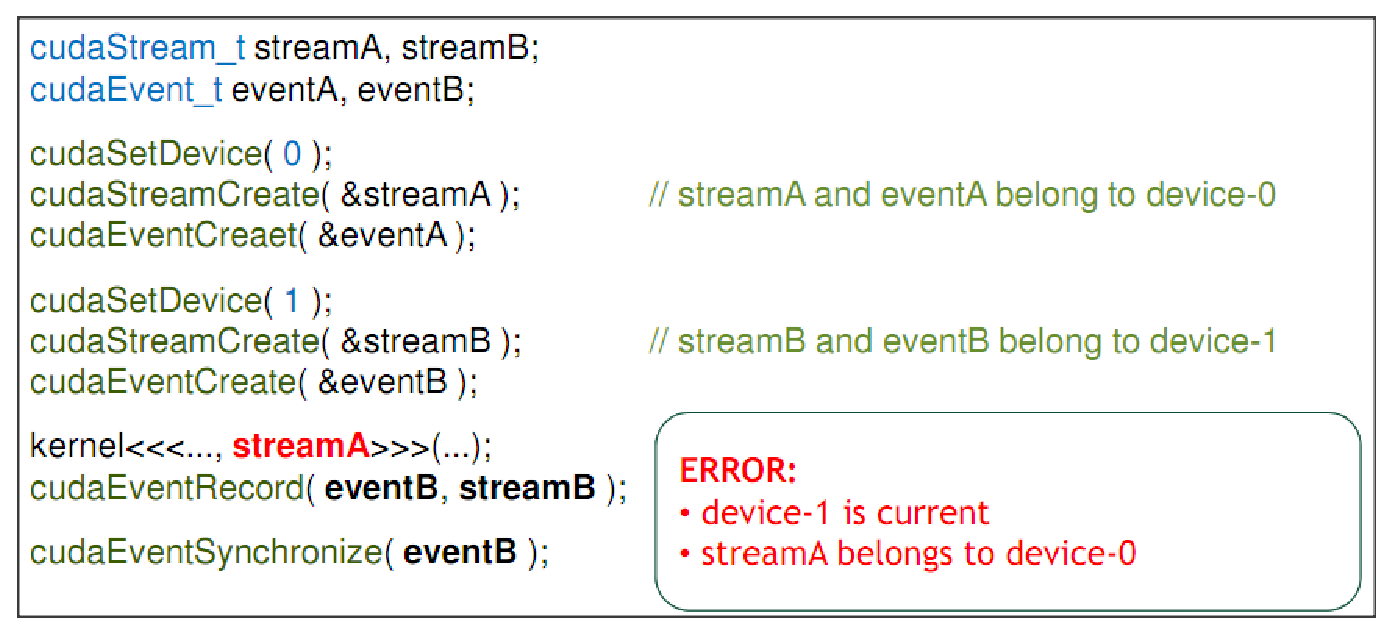
\includegraphics[height=6cm,
    angle=0]{./images/CUDA4_ex_wrongstream.eps}}
  \caption{Kernel evokation cannot be issued}
  \label{fig:CUDA4_wrongstream}
\end{figure}


Single processor (can be multiple cores) and multiple GPU: the problem
is we share the bus.

So multiple processor and multiple GPU: the GPUs use different PCI
address buses. Yet, the host memory is at different distance for
different devices. You need to take care of choosing the right CPU and
right core to use. HOW ??? (TUAN) to schedule CPU threads to the core
next to the GPU you're using??? - ANSWER: run multiple test and see
which core near which GPU by switching different GPU devices at
different test; and then call xfinity call ... (see sample codes)


So, the rule of thumb is to use as many CPU threads as necessary (to
reduce latency between communication, spin-locking to wait for kernel
execution, and direct access to device memory.


Summary: we need only a single CPU thread. However, it can loose some
concurrency. 



\subsection{CUDA driver API 4.0 }
\label{sec:GPUs_driverAPI4.0}

Prior to CUDA 4.0, we use push/pop mechanism \verb! cuCtxPushCurrent()! and 
\verb!cuCtxPopCurrent()! to iterate through each device. Example:
\begin{verbatim}
 push(ctx0); pop(ctx0); push(ctx1); pop(ctx1)
\end{verbatim}

A new mechanism, set/get interface, gives more convenient. This is the newly
added mechanism in CUDA 4.0 with \verb!cuCtxSetCurrent()! and
\verb!cuCtxGetCurrent()!.


Chapter 8 (best CUDA programming practice)





\subsection{GPUDirect 1.0 + Infiniband + MPI}
\label{sec:GPUDirect-v1}

We can do the same with Sect.\ref{sec:GPUs_GPUDirect1}. GPUDirect 1.0 P2P will
continue to work on Fermi-based GeForce, Tesla and Quadro GPUs in the CUDA 4.0
production release. However, two GPUs on the same node now can communciate
directly (Sect.\ref{sec:GPUs_GPUDirect2}).

This requires Mellanox OFED 1.5.x and above (Sect.\ref{sec:OFED}).

\subsection{CUDA 4.0: GPUDirect 2.0 with UVA (multiple GPUs within node)}
\label{sec:GPUs_GPUDirect2}
\label{sec:GPUDirect-v2}

\begin{figure}[hbt]
  \centerline{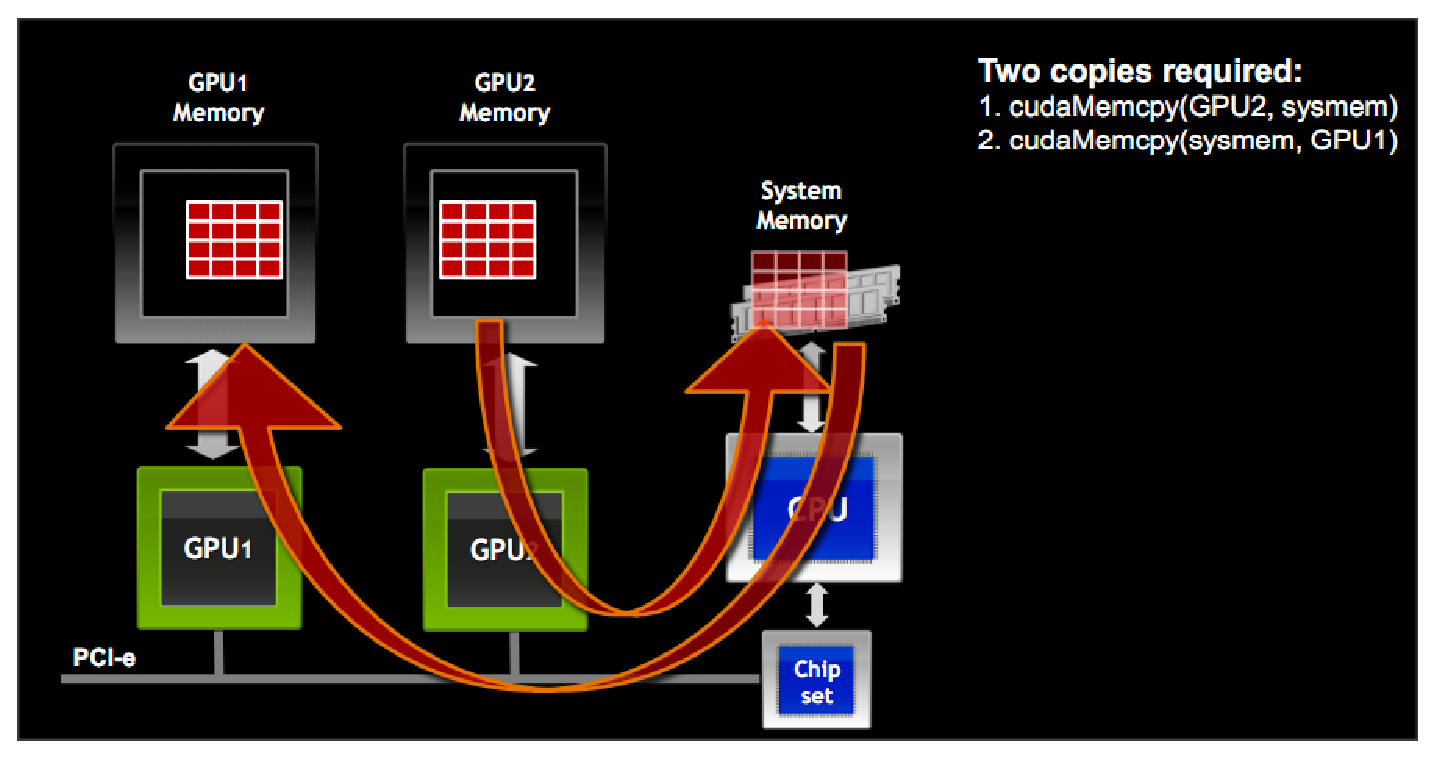
\includegraphics[height=5cm,
    angle=0]{./images/GPUDirect1.eps}}
\caption{Before GPUDirect 2.0, two GPUs on the same nodes can only communicate
to each other via CPU memory}
\label{fig:2GPU_communicate}
\end{figure}

Before CUDA 4.0, two GPUs on the same node need to use an intermediate buffer to
exchange data, Fig.\ref{fig:2GPU_communicate}. Since CUDA 4.0 and Fermi GPUs,
UVA (Unified Virtual Addressing) is introduced. GPUDirect 2.0 is built on top of UVA.
\textcolor{red}{Rather than an upgrade, GPUDirect 2.0 is a new standard designed
for applications that use multiple GPU within a node, without needing to use
Infiniband as GPUDirect 1.0}. 

With UVA, the physical memories of the CPU and GPU are mapped to a single
virtual space address. So, two location of the data (in CPU or GPU1 or GPU2),
can be checked duringe execution. So, it's possible to pass either GPU memory
pointers or CPU memory pointers to MPI. So, GPU1 can access data in GPU memory
directly, i.e. zero-copy and the pointers can be passed to MPI functions. Since
CUDA 4.0, GPUDirect 2.0 support not only (1) peer-to-peer memory access, but
also (2) peer-to-peer data transfer, with R270 drivers or later. Limitation,
GPUDirect 2.0 currently works on 64-bit system only (Linux or Windows).

To do multiple-GPU in one node, here is the code
\footnote{\url{https://www.pgroup.com/lit/articles/insider/v3n3a2.htm}}. The
program is typically working on a spatial domain, where the program, at each
tie-step, loops through each point (cell) in a grid to evaluate the contents in
the point. While each point can be evaluated in parallel, the process must
exchange boundaries (i.e. halos) when the grid is decomposed across multiple
processes; each process link to one GPU. So, in this case, we have 2 processes,
and two GPUs on the machine.
\begin{enumerate}
  \item Double-buffers is used: one to hold the current state, one to hold the
  new state
  \item Initialize the values at each grid-point
  \item Enter the time-loop
  \begin{itemize}
    \item Update to buf2 using buf1
    \item Assign: buf1 = buf2
  \end{itemize}
  \item End the simulation
\end{enumerate}

CPU: The rule is the value of the current cell is determined by the value of the
neighboring cells. Each cell can get ether 0 (die) or 1 (alive).
\begin{verbatim}
      do, while (count.lt.10.and.steps.lt.10000)
          call life(A,B,Nx,Ny)
          A=B
          alive = sum(A)
          if (prev.lt.(alive+2).and.prev.gt.(alive-2)) then
              count = count + 1
          else
              count = 0
          endif
          prev = alive
          steps = steps + 1
      end do
\end{verbatim}

1 GPU:
\begin{verbatim}
dOld=A
     dNew=0
     dimBlock = dim3(XBLOCKSIZE,YBLOCKSIZE,1)
     dimGrid = dim3((Nx+XBLOCKSIZE-1)/XBLOCKSIZE,(ny+YBLOCKSIZE-1)/YBLOCKSIZE,1)
     do, while (count.lt.10.and.steps.lt.10000)
         call life_kernel<<<dimGrid,dimBlock>>>(dOld,dNew,Nx,Ny)
         call partsum<<<SUMSIZE,SUMSIZE>>>(dNew,dPsum,dim)
         call finalsum<<<1,SUMSIZE>>>(dPsum,dFinalSum,dim)
         alive = dFinalSum
         if (prev.lt.(alive+2).and.prev.gt.(alive-2)) then
            count = count + 1
         else
            count = 0
         endif
         prev = alive
         steps = steps + 1
     end do
\end{verbatim}

2 GPUs + MPI: one process one GPU. Once a CUDA context is created, we cannot
change the GPU
\begin{verbatim}
program MAIN
use mpi
use cudafor
implicit none


! make sure there is GPUs 
! get the number of devices on this node
     ierr=cudaGetDeviceCount(numdev)

     if (numdev .lt. 1) then
       print *, 'ERROR: There are no devices available on this host.  ABORTING.', myrank
       stop
     endif

! MPI: there can be more than one MPI-process per node, i.e. nprocs
! determine who's on this node
     numlocal=0
     localprocs=0
     do i=1,nprocs
       if (hostid .eq. hostids(i)) then
         localprocs(i)=numlocal
         numlocal = numlocal+1
       endif
     enddo

! The number of devices should be greater or equal the number of MPI-process
     if (numdev .lt. numlocal) then
       if (localprocs(myrank+1).eq.1) then
         ! print the message only once per node
         print *, 'WARNING: The number of local process is greater than the number of &
         devices.', myrank
       endif
       mydev = mod(localprocs(myrank+1),numdev)
     else
       mydev = localprocs(myrank+1)
     endif

     ierr = cudaSetDevice(mydev)

! A CUDA context is created

     
\end{verbatim}

2 GPUs + 1 process: Sect.\ref{sec:GPUs_cuda4_singlethread}


\subsubsection{Limitations}

GPUDirect 2.0 is designed to work with PCI-E Gen.2 communication protocol, but
not compatible with QPI technology (see Sect.\ref{sec:QPI_IOH}).
Thus, in order for it to works with maximum performance, 2 GPUs need to connect
to the same IOH, Fig.\ref{fig:GPUDirect2.0_IOH}. A single IOH (I/O hub) can
support up to 36 PCI-E lanes. It's recommended to use 16-lanes for each GPU. So,
maximum 2 GPUs can connect to a single IOH. Also, GPUDirect 2.0 only support
Tesla (or Fermi) or Quadro cards, not Geforce.


\begin{figure}[hbt]
  \centerline{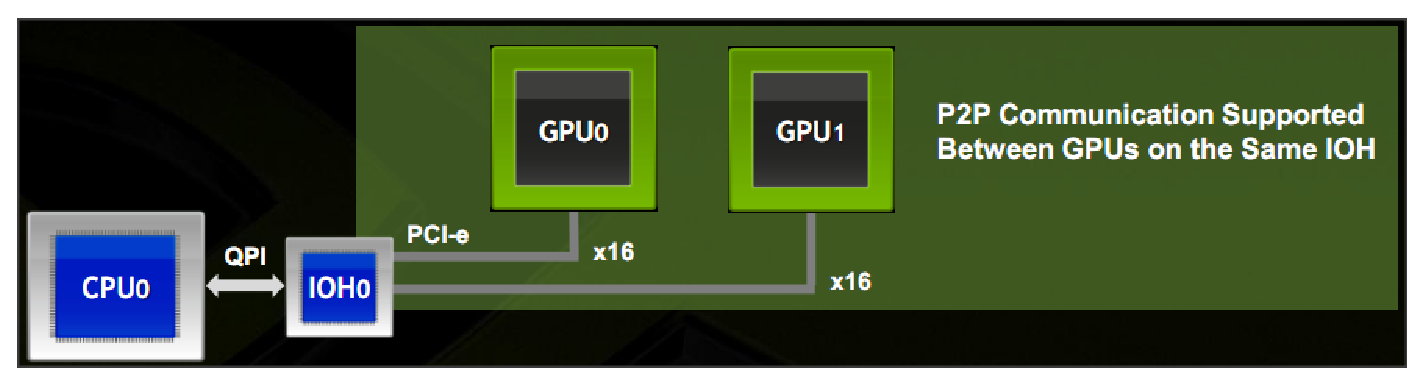
\includegraphics[height=3cm,
    angle=0]{./images/IOH_single.eps}}
\caption{P2P support GPUs connecting to a single IOH only (CUDA 4.0)}
\label{fig:GPUDirect2.0_IOH}
\end{figure}

There is, however, a problem. In NUMA architecture, where each CPU connects to
its own IOH. Then, one CPU can connect fast to two GPUs, and one CPU connect
slower through QPI via 2 IOHs, Fig.\ref{fig:IOH_P2P}. A current solution is to
use PCI-E switch, Fig.\ref{fig:QPI_IOH}, and two CPUs should connect to the
same IOH, Fig.\ref{fig:QPI_PCIswitch}.

\begin{figure}[hbt]
  \centerline{\includegraphics[height=3cm,
    angle=0]{./images/QPI_PCIswitch.eps}}
\caption{Dual-CPU system with single IOH}
\label{fig:QPI_PCIswitch}
\end{figure}

\begin{itemize}
  \item Direct access (Sect.\ref{sec:CUDA4_peer2peer-access})
  \begin{enumerate}
  \item GPU0 can read/write GPU1 global memory
  \item GPU0 access data in L2 cache of the GPU1
  \end{enumerate}
  
  \item Direct transfer (Sect.\ref{sec:CUDA4_peer2peer-copy})
  \begin{enumerate}
    \item \verb!cudaMemcpy! can copy data from GPU0 to GPU1 direct via DMA.
    \begin{lstlisting}
    cudaMemcpy(GPU2, GPU1)
    \end{lstlisting}
    \item works transparently with CUDA Unified Virtual Addressing (UVA)
    (Sect.\ref{sec:})
  \end{enumerate}
\end{itemize} 

\begin{figure}[hbt]
  \centerline{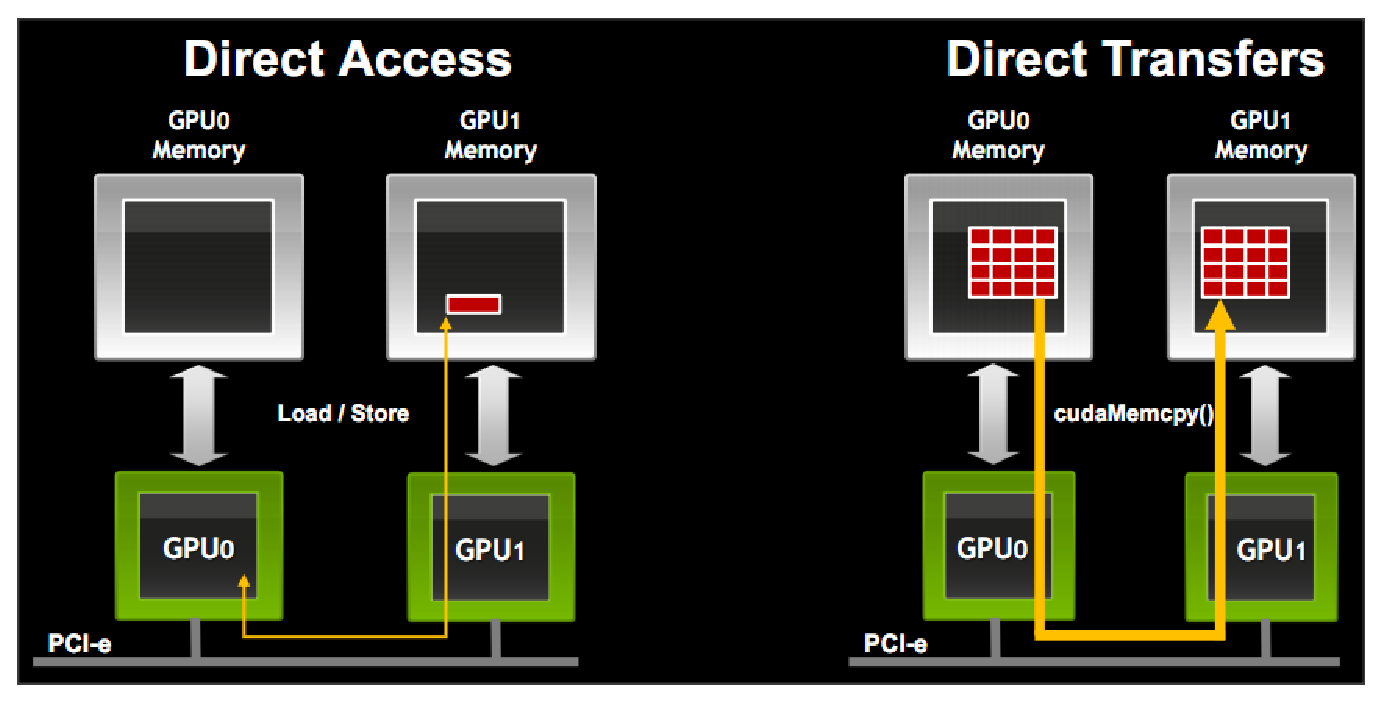
\includegraphics[height=5cm,
    angle=0]{./images/GPUDirect2.eps}}
\caption{GPUDirect 2.0}
\label{fig:GPUDirect2.0}
\end{figure}

In GPUDirect 2.0, the system needs 2 Fermi GPUs connecting to the same IOH, with
Linux kernel 2.6.15 or later (no Linux kernel patch is required) or Windows TCC
64-bit. Then, we need to set the environment variable
\begin{lstlisting}
CUDA_NIC_INTEROP = 1
\end{lstlisting}
To use, we need all CUDA pinned memory to be allocated first in user-mode as
pageable memory. Then, CUDA and third-party driver will pin and share the page
via \verb!get_user_pages()!. 

\begin{framed}
Chipsets using QPI does not support full PCIe Gen-2
standard for P2P communication across IOH; so GPUDirect 2.0 doesn't work with
Intel IOH.
CUDA 4.0 final version disable P2P across IOH. Thus, to use GPUDirect 2.0, GPUs
should be on the same IOH, Fig.\ref{fig:QPI_IOH} and Fig.\ref{sec:IOH_P2P}. So,
when P2P is not available, cudaMemcpy falls back to Device-to-Host-to-Device.

A highest performance can be achieved when the CPU process running on a CPU and
use the closest GPU. To lock a CPU thread to a socket that's closest to a GPU's
IOH chip, we use commands like {\bf taskset} and {\bf numactl},
\verb!GOMP_CPU_AFFINITY!, \verb!KMP_AFFINITY!, etc. to place processes and
memory carefully to get highest performance access to
GPUs\footnote{\url{http://sagivtech.com/contentManagment/uploadedFiles/fileGallery/GTS_Israel_2011/GPU_Computing_on_Clusters.pdf}}.
\end{framed}

\begin{figure}[hbt]
  \centerline{\includegraphics[height=5cm,
    angle=0]{./images/QPI_IOH.eps}}
  \centerline{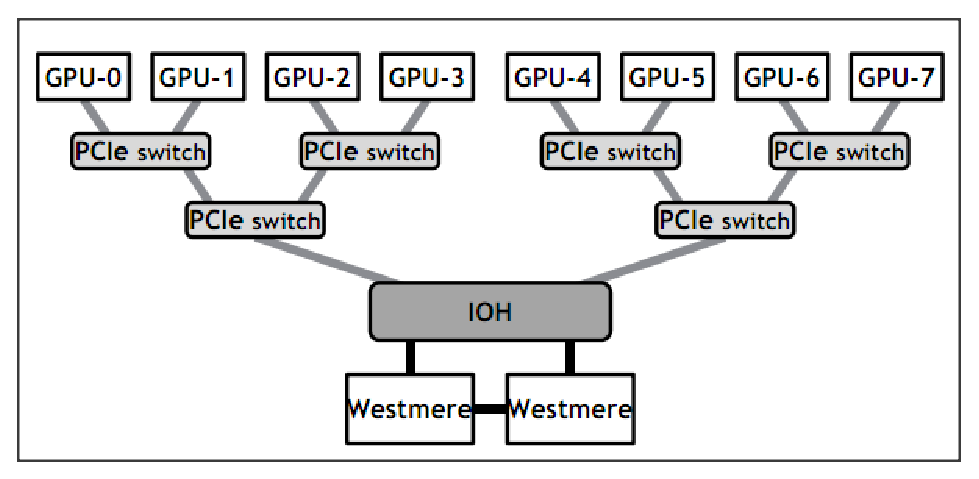
\includegraphics[height=5cm,
    angle=0]{./images/IOH_8GPU.eps}}
\caption{(A) QPI and IOH; (B) A node with 8 GPUs on a single IOH}
\label{fig:QPI_IOH}
\end{figure}

To check if a GPU configuration work on a single IOH or not, we
run\footnote{\url{http://forums.nvidia.com/index.php?showtopic=197840}}
\begin{verbatim}
lspci -tv
\end{verbatim}
If it shows
\begin{lstlisting}
 \-[0000:00]-+-00.0  Intel Corporation 5520 I/O Hub to ESI Port
             +-01.0-[0000:01]--
             +-03.0-[0000:02]--+-00.0  nVidia Corporation Device 06c0
             |                 \-00.1  nVidia Corporation Device 0be5
             +-07.0-[0000:03]--+-00.0  nVidia Corporation Device 06d1
             |                 \-00.1  nVidia Corporation Device 0be5
             +-13.0  Intel Corporation 5520/5500/X58 I/O Hub I/OxAPIC Interrupt Controller

\end{lstlisting}
then it works. Another example:
\begin{lstlisting}
 \-[0000:00]-+-00.0  Intel Corporation 5520 I/O Hub to ESI Port
             +-01.0-[0000:03]----00.0  Mellanox Technologies MT26428 [ConnectX VPI PCIe 2.0 5GT/s - IB QDR / 10GigE]
             +-03.0-[0000:0f]--+-00.0  nVidia Corporation Device 06d1
             |                 \-00.1  nVidia Corporation Device 0be5
             +-07.0-[0000:28]----00.0  nVidia Corporation G96 [Quadro FX 380]

\end{lstlisting}


\begin{figure}[hbt]
  \centerline{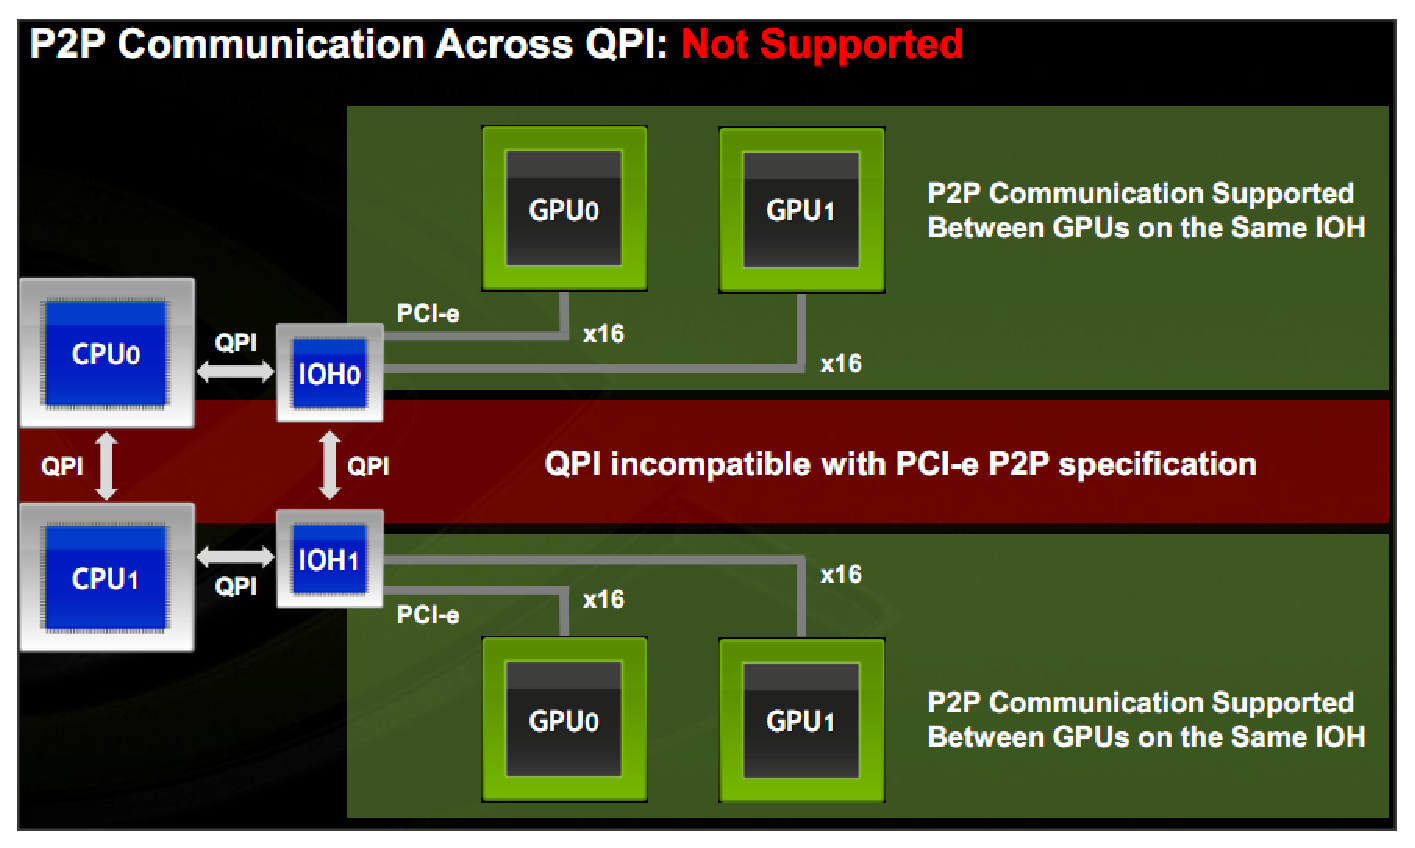
\includegraphics[height=5cm,
    angle=0]{./images/IOH_across.eps}}
\caption{GPUDirect 2.0 is not compatible with QPI. Thus the bandwidth is slow}
\label{fig:IOH_P2P}
\end{figure}

Currently, P2P Access is supported for GPUs in the same node. For GPUs in
different nodes, communicating across QPI (Intel QuickPath Interconnect) bus is
not available yet, i.e. a future feature. NOTE: QPI is incompatible with PCIe-
P2P specification.

References:
\begin{itemize}
  \item \url{http://developer.nvidia.com/gpudirect}
\end{itemize}


\section{Multi-GPU CUDA 5.x + Kepler}

GPUDirect RDMA (Remote Direct Memory Access) will be available since CUDA
5.0 (release in September, 2012). This allows direct memory access from one node
to GPU in another node, Fig.\ref{fig:GPUDirect_RDMA}.

\begin{figure}[hbt]
  \centerline{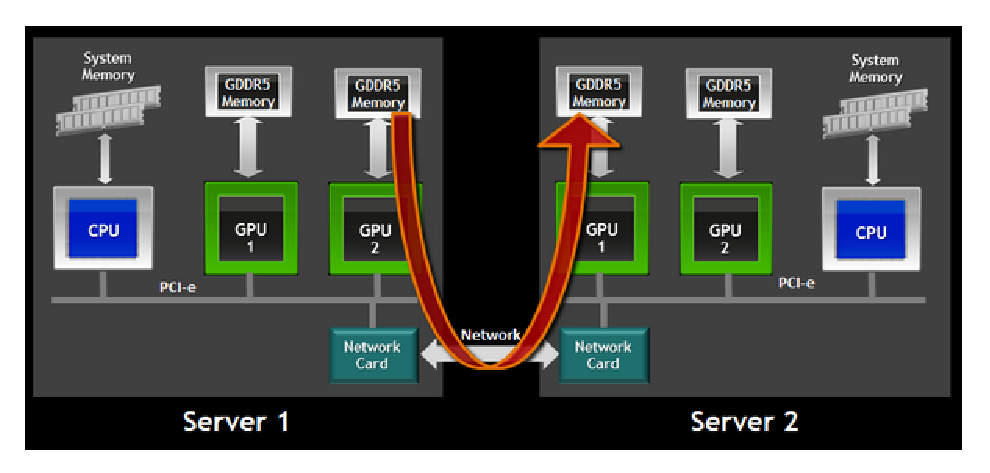
\includegraphics[height=5cm,
    angle=0]{./images/GPUDirect_RDMA.eps}}
  \caption{GPUDirect with RDMA support (CUDA 5.0)}
  \label{fig:GPUDirect_RDMA}
\end{figure}


\subsection{GPUDirect RDMA}
\label{sec:GPUDirect-v3}

GPUDirect RDMA alpha release on Q4'2013 for Kepler-class GPU and CUDA 5.0.
This enable direct memory access, i.e. zero-copy,  for communication between the
GPU and a peer device using standard features of PCI Express. 
The devices (GPU-GPU, GPU-thirdparty device) must share the same upstream root
complex, i.e. same PCI Express root. 

 Using
RDMA, network adapters can directly read/write data from/to GPU device memory, without using 'pinned'
buffers, Fig.\ref{fig:GPUDirect_RDMA}.

GPUDirect RDMA provides direct P2P (Peer-to-Peer) data path between GPU memory
to/from Mellanox HCA devices, i.e. completely bypass the host memory. To get it
working, we needs
\begin{enumerate}
  \item Mellanox ConnectX-3 or ConnectX-3 Pro or Connect-IB
  
Sect.\ref{sec:GPUDirect}  
  
  \item GPU K-series (K10, K20, K40): with Nvidia driver 331.20 or later.
  \item Mellanox OFED 2.1 or later
  \item Nvidia CUDA 5.0: need to use patch
  \item Nvidia CUDA 5.5 or later: final release is based on CUDA 6.0 (October
  2014) 
\end{enumerate}
 
 
NOTE:
\url{http://on-demand.gputechconf.com/gtc/2013/webinar/gtc-express-gpudirect-rdma.pdf}
\begin{enumerate}
  \item P2P write: 5.2 GB/s
  \item P2P read: $<$ 1.0 GB/s
\end{enumerate}

\url{http://www.mellanox.com/page/products_dyn?product_family=116&mtag=gpudirect}

\subsection{MPI with GPUDirect RDMA}

MPI implementations that supports GPUDirect RDMA is MVPICH from Ohio State
University (MVAPICH2.1.9-GDR). MVAPICH2-GDR is built upon MVAPICH2 software
stack. MVAPICH2-GDR 2.0b  (\verb!G!PU\verb!D!irect \verb!R!DMA) is derived from
MVAPICH2 2.0b (MPI-3 implementation based on MPICH ADI3 layer) and was available for download:
\url{http://mvapich.cse.ohio-state.edu/download/mvapich2gdr/}

\begin{enumerate}
  \item RDMA-based inter-node point-to-point communication: GPU-GPU, GPU-Host,
  Host-GPU using GPUDirect RDMA and pipelining
  \item Multi-rail support intern-node point-to-point GPU communication
  \item intra-node point-to-point communication multi-GPU adapters/node
  (GPU-GPU, GPU-Host, Host-GPU) using CUDA IPC (since CUDA 4.1) and pipelining
  \item Automatic communication channels: different GPU communication modes
  (Device-Device (DD), HH and HD) in different configurations (intra-IOH and
  inter-IOH)
  
  \item AlltoAll and Allgather collective communication from GPU device buffers
  
  \item Efficient vector, hindexed datatype processing on GPU buffers
  
  \item Dynamic CUDA initialization: support GPU device selection after
  \verb!MPI_Init()!
  \item Support non-blocking streams in asynchronous CUDA transfer for better
  overlap
  \item Efficient synchronizing using CUDA events for pipelined device data
  transfer
  \item Support running on heterogeneous clusters with GPU and non-GPU nodes
\end{enumerate}


To use we need 
\begin{enumerate}
  \item GPUDirect RDMA driver from Mellanox (ConnectX-3 or ConnectX-IB)
  
  \item MVAPICH2-GDR from OSU
  
  \item Trigger the feature with a runtime parameter \verb!MV2_USE_CUDA=1! and
  to activate GDR functionality, use one more runtime parameter
  \verb!MV2_USE_GPUDIRECT=1!
\end{enumerate}

\section{Inter-device coupling/synchronization (event,stream)}
\label{sec:GPUs_device-coupling}

CUDA streams and CUDA events are per device; thus we can synchronize stream and
events, regardless of the active GPU. To synchronize across streams on different
CUDA context, including streams from different devices, we use
\verb!cudaStreamWaitEvent()! with \verb!cudaEventRecord()!.


Example: consider an iterative application that executes kernels on two or more 
devices, synchronizes the devices, exchanges the boundary (halo) data among the 
devices, synchronizes again, and then repeats

\begin{lstlisting}
for (int i=0; i<iterations; i++)
{
    // Launch kernels on each device and record events to let
// us know when the kernels launches complete
    cudaSetDevice(0);
   kernel<<<grid, block, 0, stream0>>>(cells0, halo0, halo1dst);
   cudaEventRecord(event0, stream0);
   
   cudaSetDevice(1);
   kernel<<<grid, block, 0, stream1>>>(cells1, halo1, halo0dst);
   cudaEventRecord(event1, stream1);
   
    // Synchronize the devices with each other
    cudaStreamWaitEvent(stream0, event1);
    cudaStreamWaitEvent(stream1, event0);
   
    // Set up asynchronous copies to transfer the boundary (halo)
// data from each device to the other, and again record events
// to signal completion.  Note: the use of cudaMemcpyAsync() in
    // this way instead of cudaMemcpyPeerAsync() assumes UVA support.
    cudaMemcpyAsync(halo1dst, halo1, size, cudaMemcpyDefault, stream0);
    cudaMemcpyAsync(halo0dst, halo0, size, cudaMemcpyDefault, stream1);
    cudaEventRecord(event0, stream0);
    cudaEventRecord(event1, stream1);
    // Synchronize the devices with each other
    cudaStreamWaitEvent(stream0, event1);
    cudaStreamWaitEvent(stream1, event0);
}
\end{lstlisting}

However, noting that you cannot use a stream from one device with an event from
another device. This code is error, Fig.\ref{fig:CUDA4_stream_event}.

\begin{figure}[hbt]
  \centerline{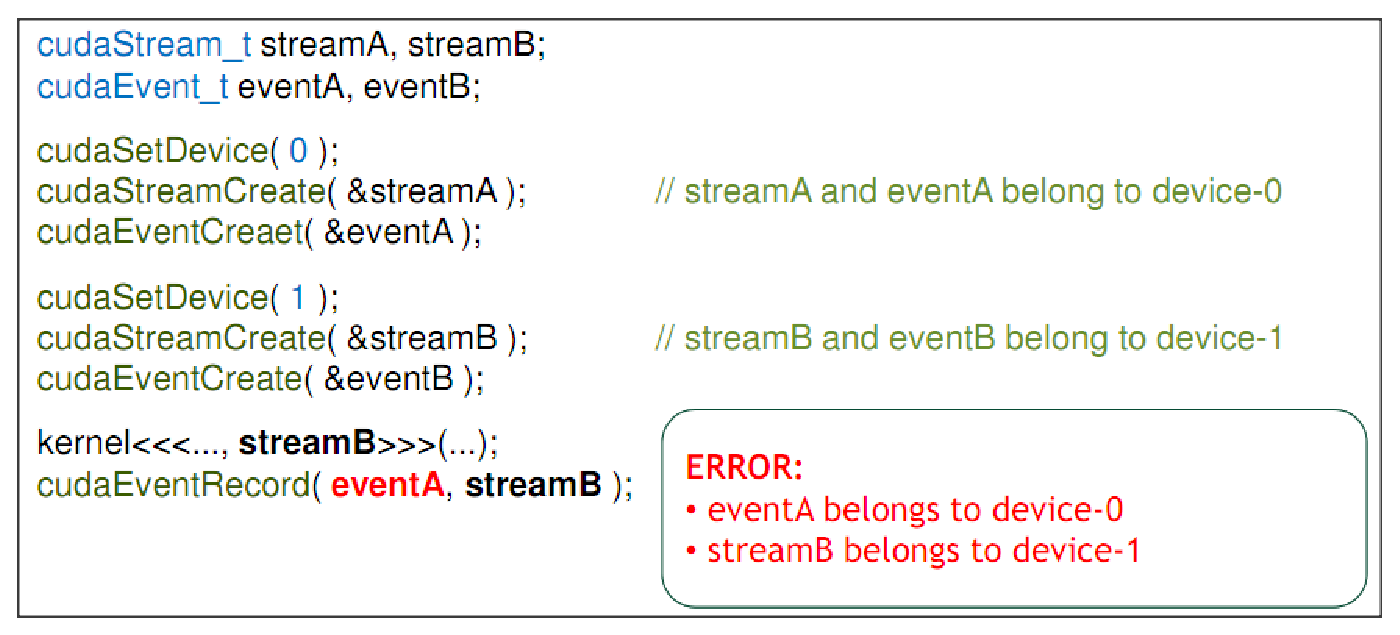
\includegraphics[height=6cm,
    angle=0]{./images/CUDA4_ex_wrongstream_event.eps}}
  \caption{ERROR when using mixed stream and event}
  \label{fig:CUDA4_stream_event}
\end{figure}

\verb!cudaEventSynchronize()! is used to wait for an event from a particular
GPU to finish before any host code or kernel code from any GPU to start. In the
following example, kernel from current device 0 have to wait for code from
device 1 to finish, Fig.\ref{fig:CUDA4_stream_wait}.

\begin{figure}[hbt]
  \centerline{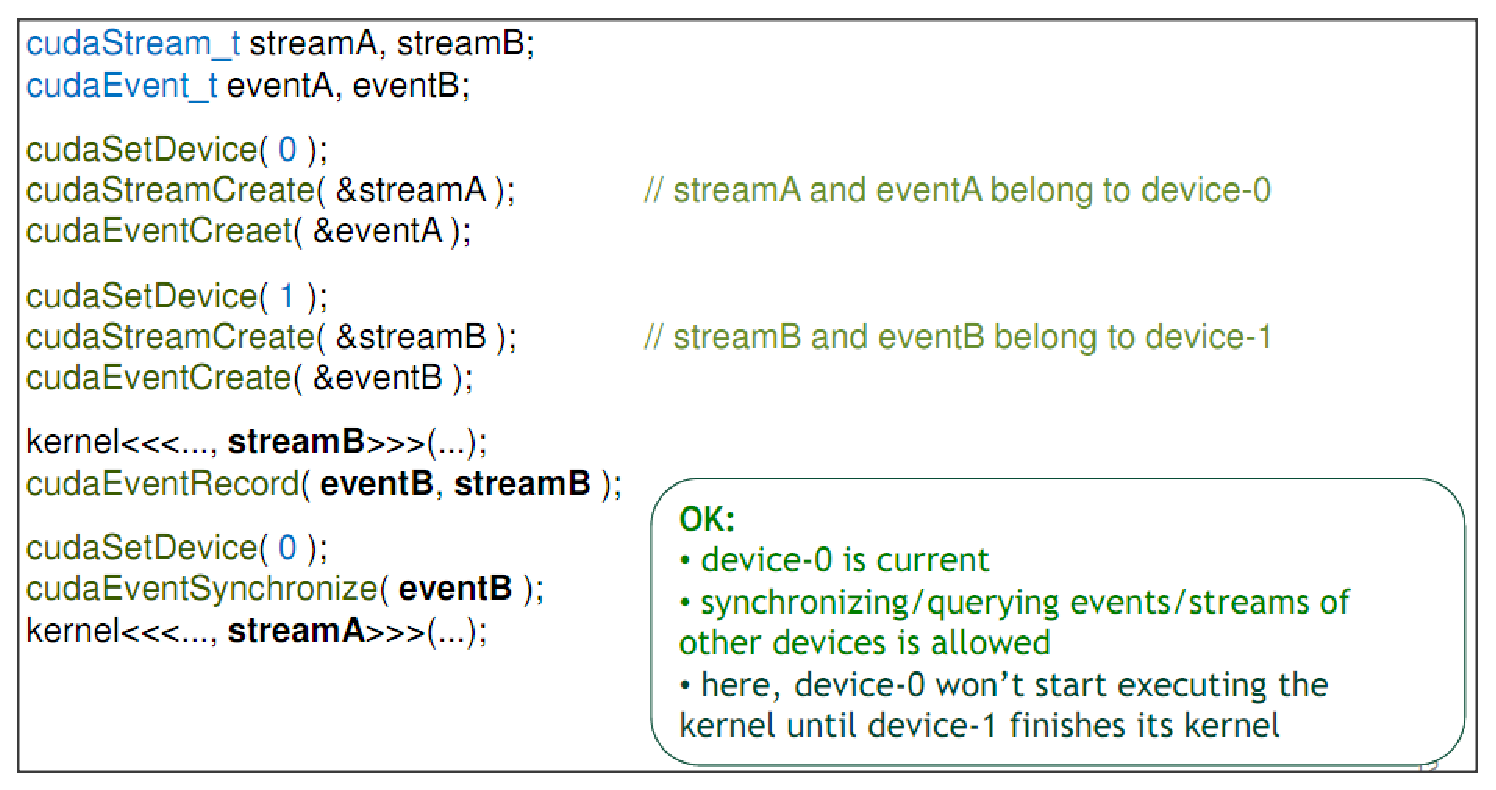
\includegraphics[height=6cm,
    angle=0]{./images/CUDA4_ex_stream_wait.eps}}
  \caption{Kernel from device 0 wait for the completion of kernel from device 1}
  \label{fig:CUDA4_stream_wait}
\end{figure}

\section{Sharing data between GPUs}
\label{sec:GPUs_share-data}

We can do via
\begin{enumerate}
  \item explicit copy via host memory (Sect.\ref{sec:GPUs_shared-host-mem})
  \item zero-copy shared host array (both devices access to the pinned memory)
  (Sect.\ref{sec:CUDA4_share_zero-copy})
  \item per-device array with peer-to-peer exchange transfer
  (Sect.\ref{sec:CUDA4_peer2peer-copy})
  \item peer-to-peer memory access (Sect.\ref{sec:CUDA4_peer2peer-access}).
\end{enumerate}

\subsection{Transfer via device-host-device memory copy}
\label{sec:GPUs_shared-host-mem}

\begin{lstlisting}
for(;;) { //time loop (simulation)
   for (int d = 0; d < devs; d++) {
     cudaSetDevice(d);
     cudaMemcpyAsync(pos[d], in, devs*bytes, H2D, s[d]);
   }
  for (int d = 0; d < devs; d++) {
     cudaSetDevice(d);
     integrate<<<b, t, 0, s[d]>>>(pos[d], otherArgs);
  }
  for (int d = 0; d < devs; d++) {
     cudaSetDevice(d);
     cudaMemcpyAsync(&out[offset[d]], pos[d], bytes, D2H, s[d]);
     cudaEventRecord(event[d], s[d]);
  }
  
  // wait for all devices
  for (int d = 0; d < devs; d++) {
     cudaEventSynchronize(event[d]);
  }
  swap(in, out); // swap host pointers
}
\end{lstlisting}

\subsection{Share via zero-copy host memory}
\label{sec:CUDA4_share_zero-copy}

Here, we don't have to copy data between GPUs; they all get access to the single
data on host page-locked memory (CUDA 3.2 and prior) or even pageable memory
(available since CUDA 4.0 with some restrictions (Sect.\ref{sec:cuda4_nocopy_pinning})) via
DMA mechanism via PCI-e Gen-2.

Data access via PCI-e Gen-2 is low bandwidth, high latency. So use if in
situations when
\begin{enumerate}
  \item copy data to GPU and access it only once AND/OR
  \item generate data on device, and copy back to host, without reuse AND/OR
  \item kernel that access memory are compute-bound, not memory-bound
\end{enumerate}

On CUDA 3.2 and prior: Sect.\ref{sec:cudaHostAlloc}

On CUDA 4.0 and later:
\begin{enumerate}
  \item register the memory (paged-locked or pageable)
  with \verb!cudaHostRegister()!. Be carefull when registering pageable memory.
  \item pass appropriate flags to cudaHostRegister(), we still need to use
  cudaHostAlloc(); but don't need to use the flags and no use
  cudaHostGetDevicePointer(). We just pass page-locked host pointers directly to
  device kernel.
\end{enumerate}


\begin{lstlisting}
// Create input and output arrays
cudaHostAlloc(&in, bytes, cudaHostAllocMapped |
cudaHostAllocPortable);
cudaHostAlloc(&out, bytes, cudaHostAllocMapped | 
cudaHostAllocPortable);
for (int d = 0; d < devCount; d++) {
   cudaSetDevice(d);
   cudaEventCreate(event[d]));
   cudaHostGetDevicePointer(&dout[d], hostPtr, 0);
   cudaHostGetDevicePointer(&din[d], hostPtr, 0);
}

for(;;) {  // simulation
   for (int d = 0; d < devs; d++) {
     cudaSetDevice(d);
     integrate<<<b, t>>>(dout[d], din[d], otherArgs);
     cudaEventRecord(event[d], 0);
   }
   
   // wait for all devices
   for (int d = 0; d < devs; d++) {
      cudaEventSynchronize(event[d]);
      swap(din[d], dout[d]); // swap in/out pointers
   }
}
\end{lstlisting}


\subsection{Peer-to-peer copy (via PCI-e Gen2)}
\label{sec:CUDA4_peer2peer-copy}

We can copy data directly from one GPU memory to another one using
\begin{itemize}
  \item Non-UVA:
  \begin{lstlisting}
  cudaError_t cudaMemcpyPeer( void * dst, int dstDevice,
                        const void* src, int srcDevice,
                        size_t count )
  \end{lstlisting}
  and
  \begin{lstlisting}
  cudaError_t cudaMemcpyPeerAsync( void * dst, int dstDevice,
                        const void* src, int srcDevice,
                        size_t count, cuda_stream_t stream = 0 )
  \end{lstlisting}
  
  \item UVA (CUDA 4.0 and later): similar to peer-to-peer access
  (Sect.\ref{sec:CUDA4_peer2peer-access}). Here, do UVA memory copy with either
  \begin{enumerate}
    \item use cudaMemcpy(\ldots, cudaMemcpyDefault)
    \item use cudaMemcpyAsync(\ldots, cudaMemcpyDefault)
    \item new APIS to use with stream: cudaMemcpyPeerAsync(), cudaMemcpyPeer()
    \begin{lstlisting}
    cudaMemcpyPeerAsync( void* dst_addr, int dst_dev, 
          void* src_addr, int src_dev, 
          size_t num_bytes, cudaStream_t stream )
    \end{lstlisting}
    with \verb!stream! must belong to the source GPU. 
  \end{enumerate}
 This function transparently use peer-to-peer DMA copy if the checking above success; and fall back to device-host-device otherwise.
  
\end{itemize}

Example:
\begin{lstlisting}
cudaDeviceCanAccessPeer(&can_access_peer_0_1, gpuid_0, gpuid_1);
cudaDeviceCanAccessPeer(&can_access_peer_1_0, gpuid_1, gpuid_0);

cudaSetDevice(gpuid_0);
cudaDeviceEnablePeerAccess(gpuid_1, 0);

cudaSetDevice(gpuid_1);
cudaDeviceEnablePeerAccess(gpuid_0, 0);

cudaMemcpy(gpu0_buf, gpu1_buf, buf_size, cudaMemcpyDefault)


cudaSetDevice(gpuid_0);
cudaDeviceDisablePeerAccess(gpuid_1);
cudaSetDevice(gpuid_1);
cudaDeviceDisablePeerAccess(gpuid_0);
\end{lstlisting}


\subsection{Peer-to-peer access (via PCI-e Gen2)}
\label{sec:CUDA4_peer2peer-access}

This requires UVA (CUDA 4.0 and later). 
With UVA, a kernel from one GPU can get access directly to data on CPU as well
as data on another GPU. For data on another GPU, it can access to global memory,
and data cached in L2 of the target GPU. This also requires 2 GPUs on the same
IOH. 

\begin{framed}
Performance expectation: 
\begin{enumerate}
  \item high bandwidth: saturate PCI-e Gen-2 can reach $\sim 6.6$ GB/s on
  single-directional transfer; for duplex it can reach $\sim 12.1$ GB/s. If
  going through the host, speed is about 4.5 GB/s.
  \item low latency: 1 PCI-e Gen-2 transaction and 1 memory fetch (take
  $\sim 2.5\mu$s)
\end{enumerate}
\end{framed}

We use \verb!cudaDeviceCanAccessPeer()! to check if a
device can get access to another one or not using GPU ID. 
\begin{enumerate}
  \item First, check if the devices if they support peer acces
  \begin{lstlisting}
  cudaDeviceCanAccessPeer()
  \end{lstlisting}
  
  \item Then, enable peer access for each pair of device using 
  \begin{lstlisting}
  cudaDeviceEnablePeerAccess(int peerDevice, unsigned int flags )
  \end{lstlisting}

\item In the kernel use the pointer to data on another device as usual
\begin{lstlisting}
cudaSetDevice(gpuid_0); SimpleKernel<<<blocks, threads>>> (gpu0_buf, gpu1_buf);
cudaSetDevice(gpuid_0); SimpleKernel<<<blocks, threads>>> (gpu1_buf, gpu0_buf);
cudaSetDevice(gpuid_1); SimpleKernel<<<blocks, threads>>> (gpu0_buf, gpu1_buf);
cudaSetDevice(gpuid_1); SimpleKernel<<<blocks, threads>>> (gpu1_buf, gpu0_buf);


................................

__global__ void SimpleKernel(float *src, float *dst)
{
const int idx = blockIdx.x * blockDim.x + threadIdx.x;
dst[idx] = src[idx];
}
\end{lstlisting}

\item We can also shutdown peer access on each device using
\verb!cudaDeviceDisablePeerAccess!. As peer-to-peer copy use more resources;
this will reduce overhead and free resources. 

The disjoint GPU-pairs can communicate without competing for bandwidth.
\end{enumerate}

\begin{framed}
NVIDIA GPUs are designed to take full advantage of the PCI-e Gen2 standard,
including the Peer-to-Peer communication, but the IOH chipset does not support
the full PCI-e Gen2 specification for P2P communication with other IOH chipsets.
If P2P doesn't work, it will fall back to device-host-device pathway.
Example: One known example system is the HP Z800 workstation with dual IOH
chipsets which can run the simpleP2P example, but bandwidth is very low (100s of MB/s instead
of several GB/s) because of the fallback path. 

Future version of GPU architecture may support communication across QPI. For
now, build multi-GPU workstation with GPUs connected to a single
IOH\footnote{\url{http://stackoverflow.com/questions/6905549/cuda-4-0-peer-to-peer-access-confusion}}

\end{framed}


\begin{figure}[hbt]
  \centerline{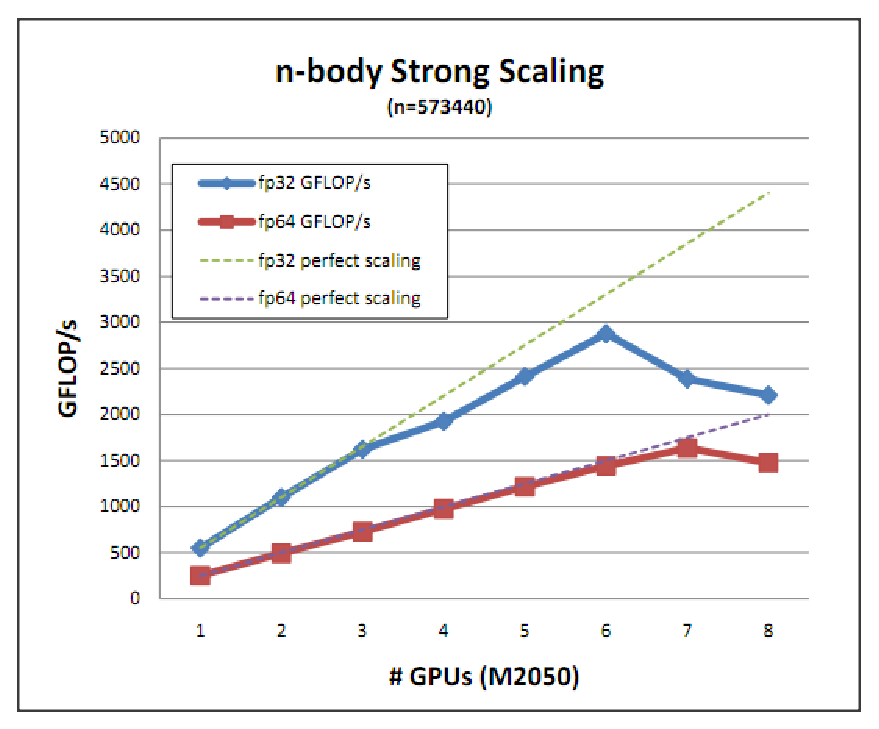
\includegraphics[height=5cm,
    angle=0]{./images/Nbody_GPUs.eps},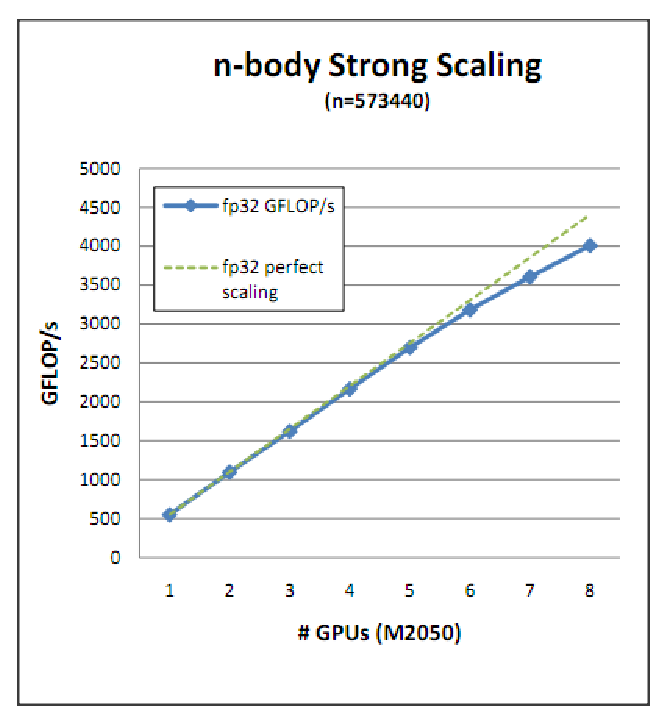
\includegraphics[height=5cm,
    angle=0]{./images/Nbody_GPUs_new.eps} }
\caption{Nbody GPUs}
\label{fig:Nbody_GPUs}
\end{figure}

Example: N-body scales well up to 4 GPUs, then performance decreases with more
GPUs, Fig.\ref{fig:Nbody_GPUs} (A). However, it's compute-bound, not
memory-bound. So, there's a chance that more than 4 GPUs can give better performance. The reason is that every thread
blocks read all positions which exceed PCI-e Gen-2 bandwidth. To resolve this, a
strategy is suggested. Suppose N=573,440, using $k$ GPU, with 256 threads/block.
Number of blocks is (N/256). Then, the amount of read per GPU is 
\begin{verbatim}
~ (N/256) * N * L2 miss rate * 16B
\end{verbatim}
Suppose the miss rate is 100\%, then 20GB read per GPU. If the miss rate is 7\%,
then 1.44GB read per GPU. Notice that PCI-e Gen-2 peak bandwidth is 8GB/s each
way, and achievable performance is 5-6GB/s. To keep the memory read below this
number, the stratey is

\begin{enumerate}
  \item each iteration, first block store positions loaded from host memory to
  device global memory
  \item then, other blocks just read from this device memory, instead of from
  host memory
\end{enumerate}
Then, PCI-e Gen-2 load is \verb!n*16B!, or with N=573,440, it requires 9MB per
GPU or 56MB per 8 GPUs. This allows one node with 8GPUs (i.e. using M2050) can
reach
4TFLOP/s\footnote{\url{http://people.maths.ox.ac.uk/gilesm/cuda/MultiGPU_Programming.pdf}},
Fig.\ref{fig:Nbody_GPUs} (B).

\section{An example of halo exchange}
\label{sec:GPUs_example}


A system (node) with 8 GPUs, Fig.\ref{sec:QPI_IOH} (B). GPUs have to exchange
halos with their left/right neighbors. A two-phase approach is used where each
GPU sends data to its right, then to its left neighbor. 

A typical pattern for multiple-GPU code is 
\begin{enumerate}
  \item compute halos (i.e. data to be sent to other GPUs)
  \item exchange data with other GPUs (using asynchronous copies). During that
  time, compute over internal data 
  \item Synchronize, before going back to step 1.
\end{enumerate}

\begin{figure}[hbt]
  \centerline{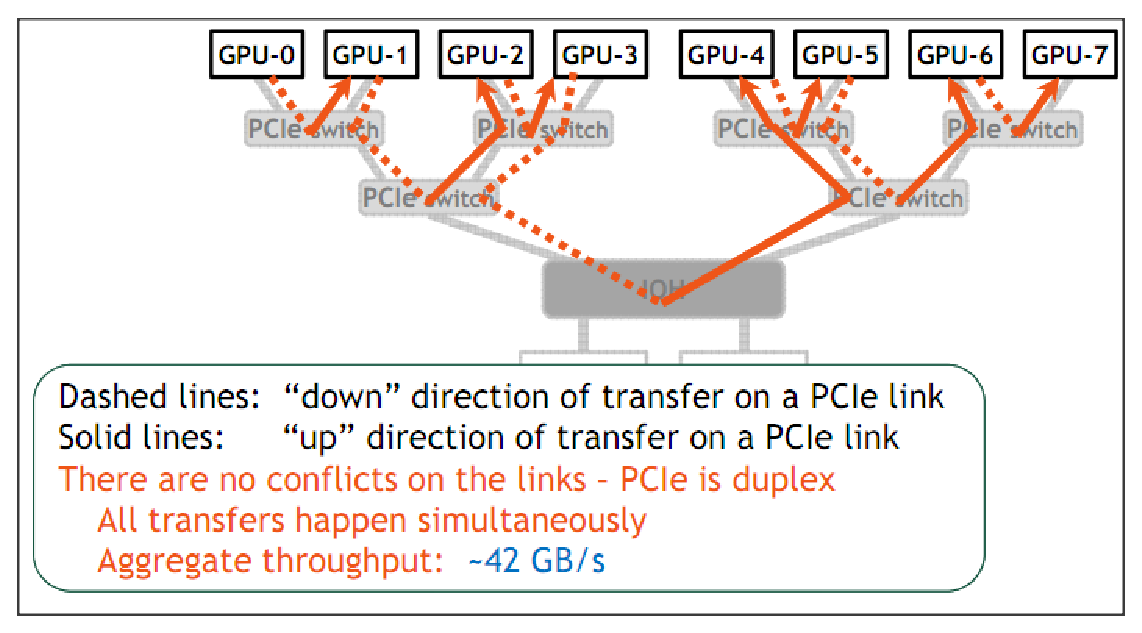
\includegraphics[height=5cm,
    angle=0]{./images/GPUs_right_step2.eps} }
\caption{GPU halo exchange}
\label{fig:GPUs_rightphase}
\end{figure}

Data copy is given as

\begin{lstlisting}

for( int i=0; i<num_gpus-1; i++ ) // "right" phase
     cudaMemcpyPeerAsync( d_a[i+1], device[i+1], d_a[i], device[i], num_bytes,
stream[i] ); 

//RECOMMEND to add a device-synchronization between the phases
cudaerr = cudaDeviceSynchronize();
 
for( int i=1; i<num_gpus; i++ ) // "left" phase
     cudaMemcpyPeerAsync( d_b[i-1], device[i-1], d_b[i], device[i], num_bytes,
stream[i] );
\end{lstlisting}
Adding the device-synchronization between phases can prevent the ``last'' device
from sending in the ``right'' phase which would cause link-contention results
is incorrect. 

NOTE: \textcolor{red}{Number of PCIe hops doesn't seem to affect througput}

\section{Speed comparison}
\label{sec:copy_speed}

\url{http://developer.download.nvidia.com/CUDA/training/cuda_webinars_multi_gpu.pdf}
\begin{enumerate}
  \item Host-2-Device on local:  5.7 GB/s
  \item Host-2-Device on remote (i.e. different data bus): 4.9 GB/s
  \item Device-2-Host on local: 6.3 GB/s
  \item Device-2-Host on remote: 4.3 GB/s 
\end{enumerate}

\section{GPU Cluster}
\label{sec:GPU_cluster}

According to Top500, 410 out of 500 are GPU clusters,
Fig.\ref{figu:GPU_cluster_hpc}, and the speed of GPU is faster than CPU,
Fig.\ref{fig:GPUvsCPU}.
Today the most powerful cluster is a GPU cluster, which was named Tianhe-1A: 2507 Petaflop, with 7168 M2050 GPUs.
National Supercomputing Center in Tianjin in China.

\begin{figure}[hbt]
  \centerline{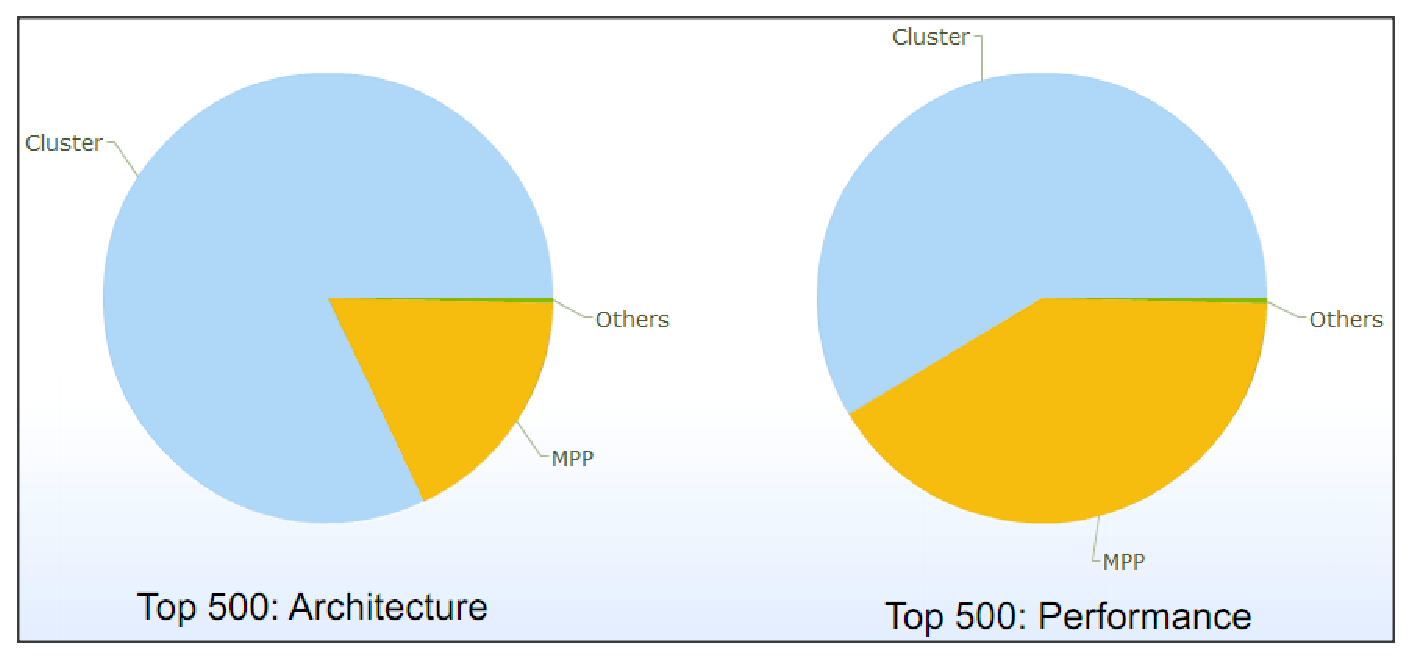
\includegraphics[height=5cm,
    angle=0]{./images/GPU_cluster_hpc.eps}}
\caption{Percents of GPU cluster in HPC}
\label{fig:GPU_cluster-hpc}
\end{figure}

\begin{figure}[hbt]
  \centerline{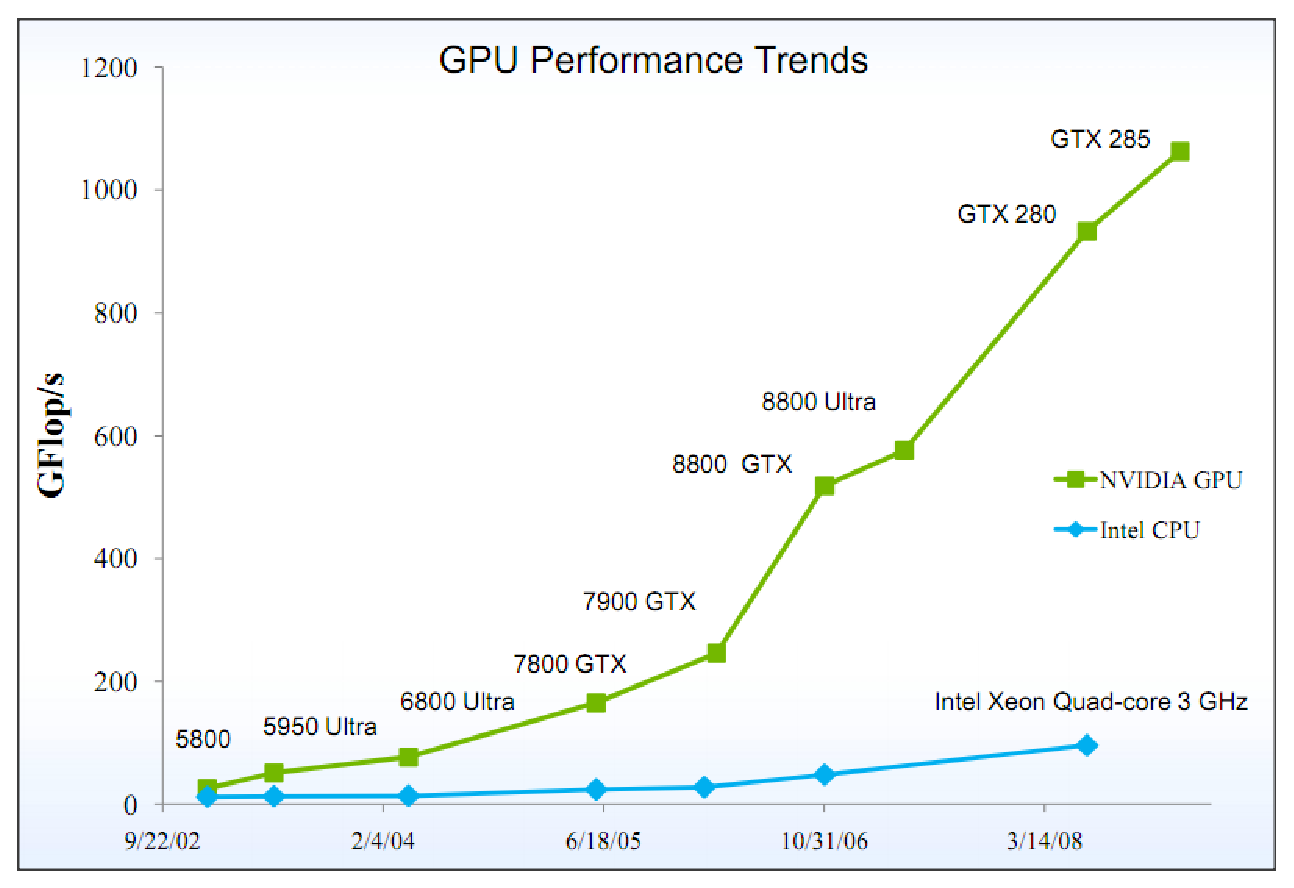
\includegraphics[height=5cm,
    angle=0]{./images/GPUvsCPU.eps}}
\caption{Speeds (in GFLOPs) comparison between CPU vs. GPU}
\label{fig:GPUvsCPU}
\end{figure}


\subsection{NCSA}
\label{sec:NCSA}

NCSA (National Center for Supercomputing Applications) has some GPU clusters,
developed from CPU clusters:
\begin{enumerate}
  \item AC: experimental system accessible to anyone interested in GPU
  computing. It has 32 servers, each one is a HP xw9400 workstation (two 2216
  AMD Opteron 2.4GHz dual socket dual core, 8GB DDR2, Infiniband QDR). Each server
  connect to a single S1070 via PCIe 1.0 x16, i.e. each AMD opteron connect to a
  switch in S1070, i.e. 32 units. IB bandwidth/host is 16 Gbit/s. Cluster
  management tool is SystemImager.
  \begin{enumerate}
    \item AC33 node: Intel core i7 8-cores using dual IOH (72 lanes PCI-E),
    connect to two S1070, PCIe-2.0 x16.
    \item AC34-AC41 nodes: A+ server (Supermicro), two AMD 6-core Istanbul, with
    IB infiniband QDR 32Gbit/s, 3 internal ATI Radeon 5870 GPUs.
    \item AC42 node: TYAN FT72-B7015 with X5680 Intel Xeon 3.33 
GHz (Westmere-EP) dual-socket hexa-core, Tylersburg-36D IOH (each IOH connect
to a single 6-core CPU), 24GB DDR3. Each IOH has 4 PCIe-2.0 switched to use 4
GTX480
  \end{enumerate}
    
\begin{figure}[hbt]
  \centerline{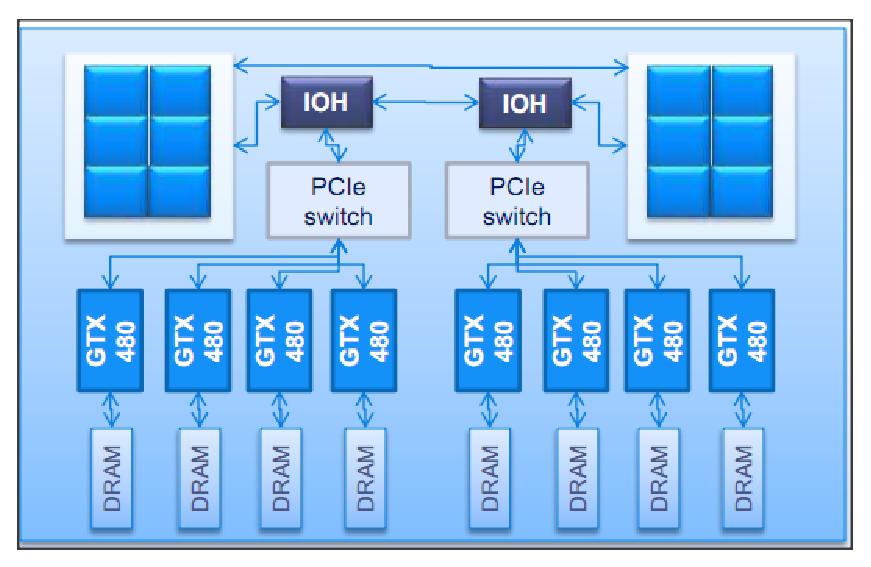
\includegraphics[height=5cm,
    angle=0]{./images/AC42_node.eps}}
\caption{AC nodes: AC42}
\label{fig:Lincoln_node.AC_node}
\end{figure}
  
  \item Lincoln: production system accessible via NCSA/TeraGrid HPC allocation.
  It has 192 servers, each one is a Dell PowerEdge 1955 Server (Intel 64
  (Harpertown) architecture 2.33GHz dual socket quad-core, 16GB DDR2, Infiniband
  SDR). Every two servers connect to a switch in S1070 via PCIe-2.0 x8, i.e. 96
  units. IB bandwidth/host is 8 Gbit/s. Cluster
  management tool is Perceus.

\begin{framed}
Workload management is Torque/MOAB. Monotoring is done by CluMon (Lincoln) and
Manual monitoring (AC). To use IB on Fermi-based card, it uses mvapich2 mpi. As
an experiment system, AC has CUDA wrapper, memtest, and power profiling. 
\end{framed}  

  \item EcoG: (\#3 on Green500 list): 128 nodes, each with EVGA P55V
  120-LFE651-TR Micro ATX Intel Motherboard (core i3 530 2.93 GHz single-socket dual-core, 4GB DDR3, PCIe-2.0
x16), IB Infiniband QDR + one Tesla C2050. 

\item Blue Waters project: Cray supercomputers equiped with Tesla GPUs.
Currently (Nov, 2011), more than 25 science teams have been selected to run on
this system (molecular dynamics and astrophysics, to earthquake engineering and
materials science). There're more than 235 Cray XE6 cabinets (based on AMD
Opteron 6200 Series processor), and more than 30 cabinets for future Cray XK6
supercomputer to equipped with next-generation Tesla ``Kepler'' architecture.

Interconnection between nodes is 3D Torus. 
\end{enumerate}

\begin{figure}[hbt]
  \centerline{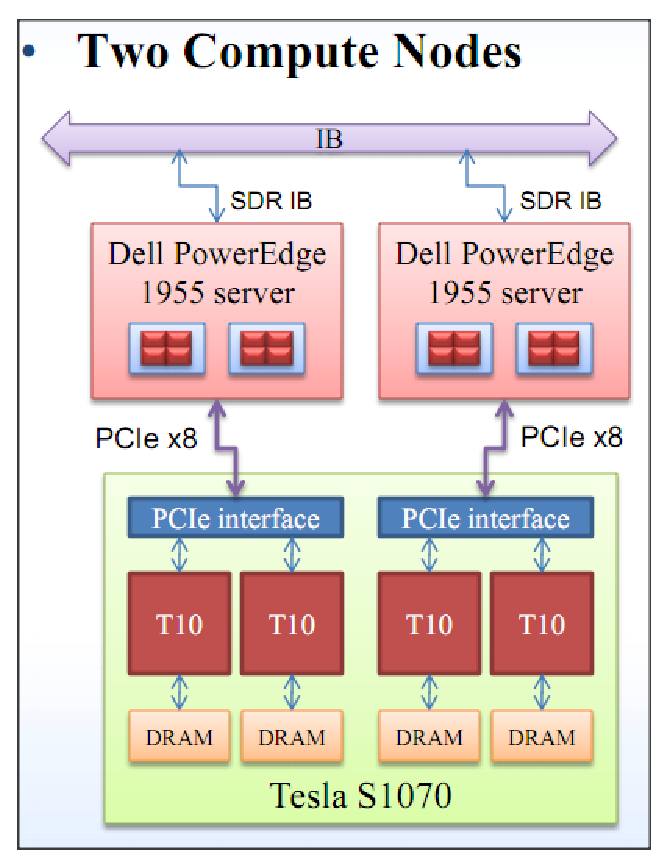
\includegraphics[height=5cm,
    angle=0]{./images/Lincoln_nodes1.eps},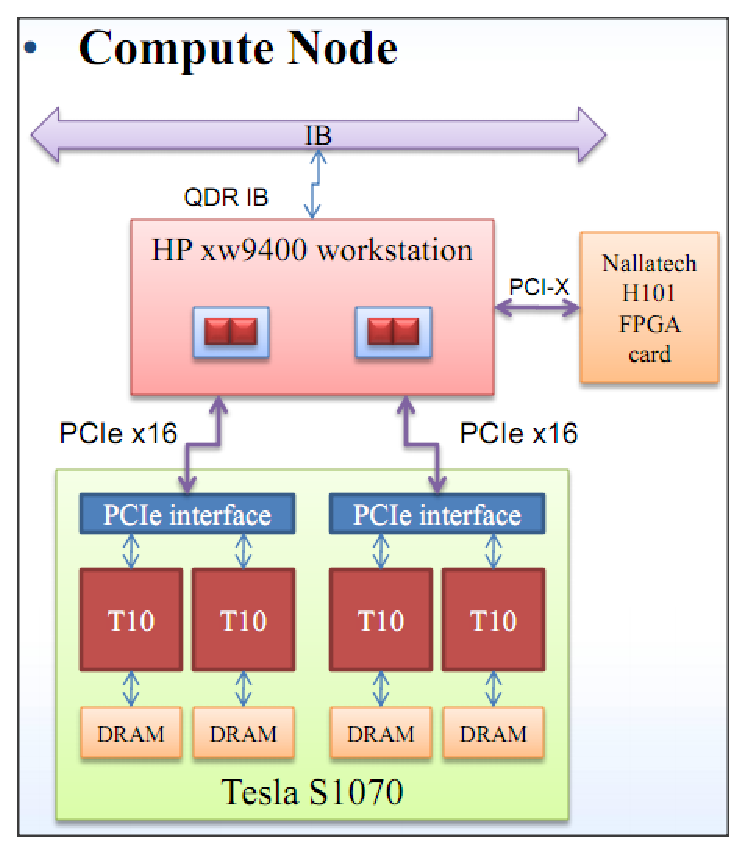
\includegraphics[height=5cm,
    angle=0]{./images/AC_nodes.eps}}
\caption{Two compute nodes in Lincoln cluster and AC cluster}
\label{fig:Lincoln_node.AC_node}
\end{figure}

Apply for AC account to use AC environment from NCSA. 
\url{http://ncsa.illinois.edu/UserInfo/Allocations/AddUserForm.html},
and refer NCSA system as ``AC cluster''. 


References:
\begin{enumerate}
  \item
  \burl{http://www.ncsa.illinois.edu/~kindr/projects/hpca/files/ppac09_presentation.pdf}
  \item
  \burl{http://www.ncsa.illinois.edu/People/kindr/projects/hpca/files/UA10_presentation.pdf}
\end{enumerate}

\subsection{NICS}
\label{sec:GeorgeTech-NSF}

NICS (National Institute for Computational Sciences) is the center formed
through the grant by NSF to University of Tenessese and its partners. Its
existing systems
are\footnote{\url{http://www.nics.tennessee.edu/computing-resources}}:
Kraken (Cray XT4) and Nautilus (SFI UltraViolet system, a single system image
with 1024 cores (Intel Nehalem EX) 4TB shared memory and 16 GPUs).

A new project, Keeneland Project has 201 Teraflop, 120-node HP SL390, each node
with two Intel XeonCPU + three nVidia C2050 GPU. The nodes are connected by IB Infiniband QDR.



\subsection{LLNL - Edge}
\label{sec:Edge}

LLNL has some clusters with equipped Tesla GPUs. Edge is for visualization and
data analysis work. Users should contact LC Hotline for access. It has
\begin{itemize}
  \item 216 nodes: 2 login nodes, and 206 batch nodes
  \item CPU: Intel Westmere
  \item GPU: Nvidia Fermi Tesla M2050 3GB DDDR5 (2 per nodes)
  \item Memory: 96GB/node, 64-bit addressing
  \item Connect: Infiniband QDR (Mellanox)
\end{itemize}

\section{GTC'12 updates}

memcpy (D2H or H2D) with  


CUDA 3.2 and earlier: Curent GPU can be changed while async calls (kernels,
memcopies) are running.


CUDA 4.x: 64-bit Linux or 64-bit (Windows with TCC driver). Fermi or later
architecture (CC 2.x or higher). A GPU thus can dereference a pointer that is an
address on another GPU or an address on host CPU. Thus, it makes multi-GPU
programming more transparent. 

The ability of accessing another GPU's addresses and do peer-to-peer (P2P)
memcpies requires peer-access to be enabled with 
\begin{verbatim}
cudaDeviceEnablePeerAccess ( peer_device, 0)

cudaDeviceCanAccessPeer ( & accessible, dev_X, dev_Y)
\end{verbatim}

GPU's DMA engine of the source data carries out the copy. So, data is
``pushed'', not ``pulled''. The calling device does nothing. 

No need to maintain a memory buffers on the host for inter-GPU exchanges. When
communication does not include IOH (i.e. GPUs connected to a PCI-e switch).
Single-direction transfer is $\sim$ 6.6GB/s ($\sim$ 12GB/s for gen3). Duplex is
$\sim 12.2$ GB/s ($\sim$ 22 GB/s for gen3 PCI-e). If going through the host,
it's only $\sim$ 5GB/s.  However, it's still lower compared to direct GPU memory
access ($\sim$ 155 GB/s for Fermi). 

GPUs are physically arranged into a trees, with GPUs connected to a PCIe switch,
with 1 PCIe switch is a node, each node has 2 GPUs. Two PCIe switchs connect to
each other via another PCI-e switch. This is the left-right approach for 4 GPUs
connecting via PCI-e switch. So, there are 3 transfer for 2 GPUs on 2 different
switches (i.e. going through switch 1, 3, and 2). The achieved throughput is
$\sim$ 15 GB/s (with 4-MB messages). 

The bus link is duplex, so as long as there is no two transfer on the same
direction the contention won't occur. This works on 4-GPU pair-wise system. The
pair-wise approach is no longer work for 8 GPUs system.
As contention can occur (if GPU1-GPU2 communicate and GPU3-GPU4 communicate,
then the bus contention occur on GPU2 and GPU3 which use the same link of the
switch).
For system with 8 GPUs, IOH is used to combine 2 trees.
The aggregated speed is $\sim$ 34 GB/s.
\begin{verbatim}
for (int i = 0; i < num_gpus-1; i++) //"right" stage (start with GPU 0)
  cudaMemcpyPeerAsync(...)
  
  for (...)
    cudaStreamSynchronize(stream[i]);
    
for (int i=1; ...)      // "left" stages (start with GPU 1)
  cudaMemcpyPeerAsync(..)
\end{verbatim}
This code prevent contention the two-stages from interfering with each other
(so increase performance from 11GB/s to 15GB/s for 4-GPU system). 

The strategy:
\begin{enumerate}
  \item Compute the halos (exchanged data)
  \item Transfer the halos. During that time, also compute the internal data.
  This can be overlapped
  \item Switch the new and old data. Synchronize before next step. 
\end{enumerate}
\begin{verbatim}
for each time step
   for each GPUs
      cudaSetDevice(gpu[i]);
      kernel<<<... stream_halo[i]>>>
      kernel<<<... stream_halo[i]>>>
      cudaStreamQuery(stream_halo[i])  
      kernel<<<  stream_internal[i]>>>
   }
   for each GPUs
      cudaMemcpyPeerAsync (..., stream_halo[i])
   for each gpu
      cudaStreamSynchronize(stream_halo[i])
   for each GPU
      cudaMemcpyPeerAsync (..., stream_halo[i])
   for each GPU
      cudaSetDevice(gpu[i])
      cudaDeviceSynchronize();
      //swap input/output pointers
\end{verbatim}


\subsection{GPUs in different nodes}

There's no PCI-e connecting two different nodes. So, data need to go through
host side first before transmitting to another node, using MPI or some socket
programming interface. 
\begin{verbatim}
cudaMemcpyAsync(, stream_halo[i])
cudaStreamSynchronize(stream_halo[i])
MPI_Sendrecv(...)
cudaMemcpyAsync(...,stream_halo[i])
\end{verbatim}
So, we need to overlap MPI and PCIe transfer
\begin{verbatim}
for each GPUs
  //send data to neighbor to the right
   cudamemcpyPeerAsync(...,stream_halo[i]);
   cudaSetDevice(gpu[num_gpus-1]);  ??? 1 or i
   cudaMemcpyAsync(...,stream_halo[num_gpus-1]);  ??? 1 or i
   
// at the same time, the host receive data from the left
// no contention to occur as it use 2 different traffic directions
for each GPU
  cudaStreamSynchronize(stream_halo[i])
  
for each GPU
   cudamemcpyPeerAsync(...,stream_halo[i]);
   cudaSetDevice(gpu[0]);
   cudaMemcpyAsync(...,stream_halo[0]);
   MPI_Sendrecv(...)
   
\end{verbatim}


Example: TTI Forward Wave Modelling (TTI FWM)
\begin{enumerate}
  \item data set is 512x512x512 cube $\rightarrow$ data size is 7GB. so need at
  least 2GPUs
  \item 3 DFD, 8th order in space, and 2nd order in time
  \item 1D domain decomposition $\rightarrow$ each GPU has 64 slices for
  the case of 8 GPUs (512/8 = 64)
\end{enumerate}
At a single time step, with single 8-GPU node
\begin{enumerate}
  \item halo computation: 1.1ms
  \item internal computation: 12.7 ms
  \item halo-exchange: 5.9ms
  \item total: 13.8ms (as halo exchanged is hidden by internal computation)
\end{enumerate}
The scaling is 12.7/12.8 $\sim $ 90\% which is high. We want to scale it down.
If each GPU gets $\sim 100$ slices, then the network is $\sim 68\%$ of all
communication times. IB QDR hides communication when each GPU gets $\sim 70$
slices. 


In the code, even though you can create multiple streams, a kernel can be
launched to a stream if the stream's GPU is current. On the other hands,
memcpies can be issued to a stream, regardless if the stream belong to the GPU
which is current or not. The driver will ensure all calls to that stream is
completed before the bytes are transfered. 

An event can only be recorded on a stream to which the GPU is current. We don't
record event that often, unless we want to benchmark. 

We can call an API to synchronize or query with any event/stream, regardless of
the state of the GPUs. 

A GPU is set to current if we call \verb!cudaSetDevice()! with the
corresponding ID. 
\begin{verbatim}
gpuID = 0
cudaSetDevice(gpuID);
cudaStreamCreate(&streamA); // associated with gpuID = 0
cudaEventCreate(&eventA);

gpuID = 1;
cudaSetDevice(gpuID)
cudaStreamCreate(&streamB); // associated with gpuID = 1

kernel<<<...., streamB>>>  //OKAY
cudaEventRecord(streamA, eventA) ;; // ERROR: gpuID=0 is not the current one

\end{verbatim}
The problem is that only one GPU can be set current at a time. A solution is
\verb!cudalpc*! APIs.

\subsection{CUDA 4.2: cudalpc* APIs}

With CUDA 4.2, there's a new set of APIs. Processes on the same can access each
other's GPU memory which  bypass communication via host with MPI.

\begin{enumerate}
  \item Process A get handle to its pointer, send it to process B
  \item Process B open the handle, get a pointer to A's address
  \item Process (or its GPU kernel) uses the pointer
  \item Process B closes the handle
\end{enumerate}

\begin{verbatim}
cudalpcMemHandle_t handle_a;
cudalpcGetMemHandle(&handle_a, (void*) d_a)

//process B
cudalpcOpenMemHandle((void**) &d_neighbr, neighbors_a,
cudalpcMemLazyEnablePeerAccess);
 // use d_neighbor like you would a locally allocated pointer
cudalcpCloseMemHandle(d_neighbor)
\end{verbatim}


\subsection{GPU-aware MPI}

\verb!mvapich, openmpi! are working to develop these APIs, which is expected to
work with C/C++, Fortran, CUDA C, CUDA Fortran, directive-based code. It can
break transfer into smaller pieces (for better performance), and pipeline the
transfer of pieces: overlap PCI-e and Net-w for all, but the first and last
piece. 

P2P path when MPI ranks are on the same node is not yet available. 


\subsection{NUMA with dual-IOH system}

CPU NUMA affects PCIe transfer throughput in a dual IO-Hub (IOH) system. This
affect any PCIe device (e.g. network cards), not just GPUs. We can lock a CPU
thread to a socket with closest GPU (HOW????). 
\begin{enumerate}
  \item local: D2H 6.3GB/s, H2D: 5.7 GB/s
  \item remote: D2H 4.3 GB/s, H2D: 4.9 GB/s
\end{enumerate}
These vary among different systems (BIOS settings and IOH chips). 

\subsection{Optimize multiple GPUs}

Using infiniband, we can do both communication with GPU in another node via
Infiniband without having to worry about memory contengtion with GPUs in that node.

Example: decompose the kernel by breaking into (n/b)$^3$ matrix multiples of
size bxb for each tile. We can use stremams to enforce the dependencies when
combining the tiles together.


Example: (Sparse cholesky) find L such that A = L$\times$L$^T$. We need to
decompose into (dpotrf, dtrsm, dsyrk). There's a severe dependencies. How to
deal with this. One strategy is non-balancing approach to avoid/reduce the
dependencies between GPU, i.e. give more work to one GPU if the work has
dependencies; then it's better if the dependencies occur within a GPU. 


In multi-GPU system, the speed is limited by the slowest one. Here is the QPI
connection for single node, or Infiniband for multiple nodes. The challenge is
how to hide this, i.e. give more computations for each GPU before communication. 


